\subsection{External Interface Requirements}
\subsubsection{User Interfaces}

\begin{figure}[H]
\centering
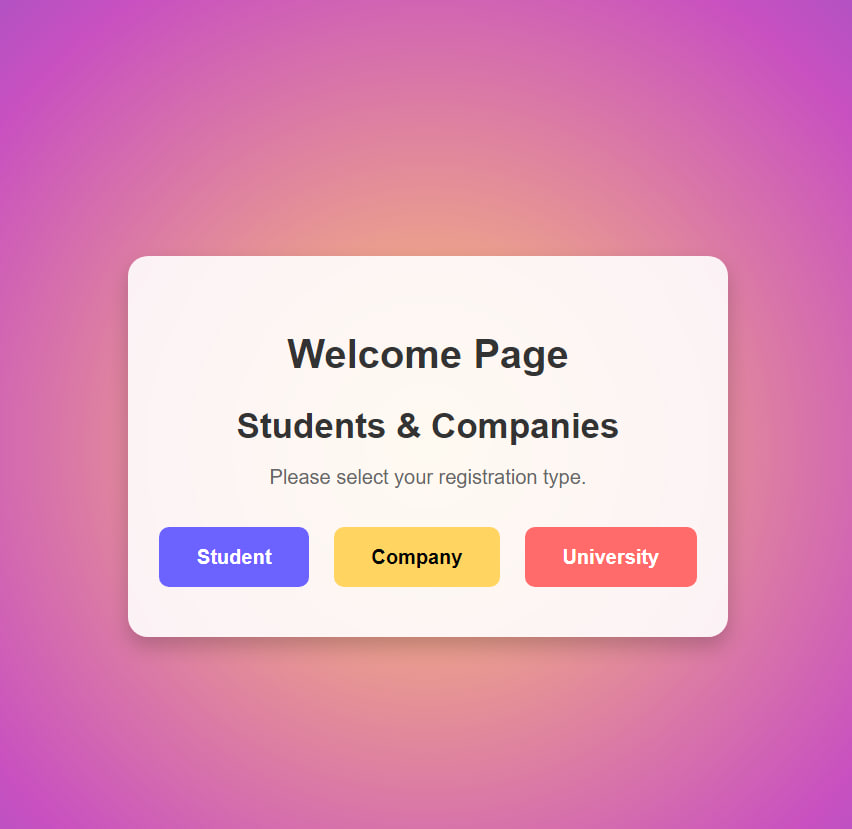
\includegraphics[width=0.8\textwidth]{Images/1.jpg}
\caption{\label{fig:metamodel1}Welcome Page.}
\end{figure}

\begin{figure}[H]
\centering
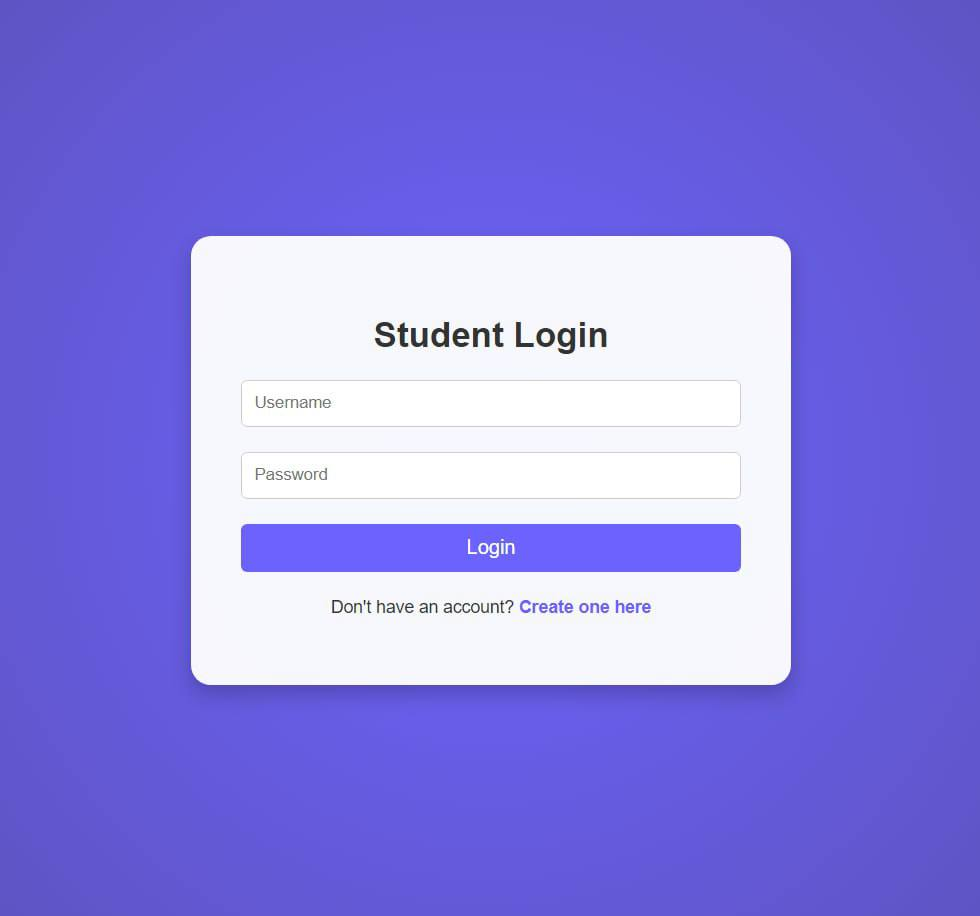
\includegraphics[width=0.8\textwidth]{Images/2.jpg}
\caption{\label{fig:metamodel2}Student Login Interface: A user-friendly login form for students to access the platform, featuring fields for username and password with a prompt for account creation.}
\end{figure}

\begin{figure}[H]
\centering
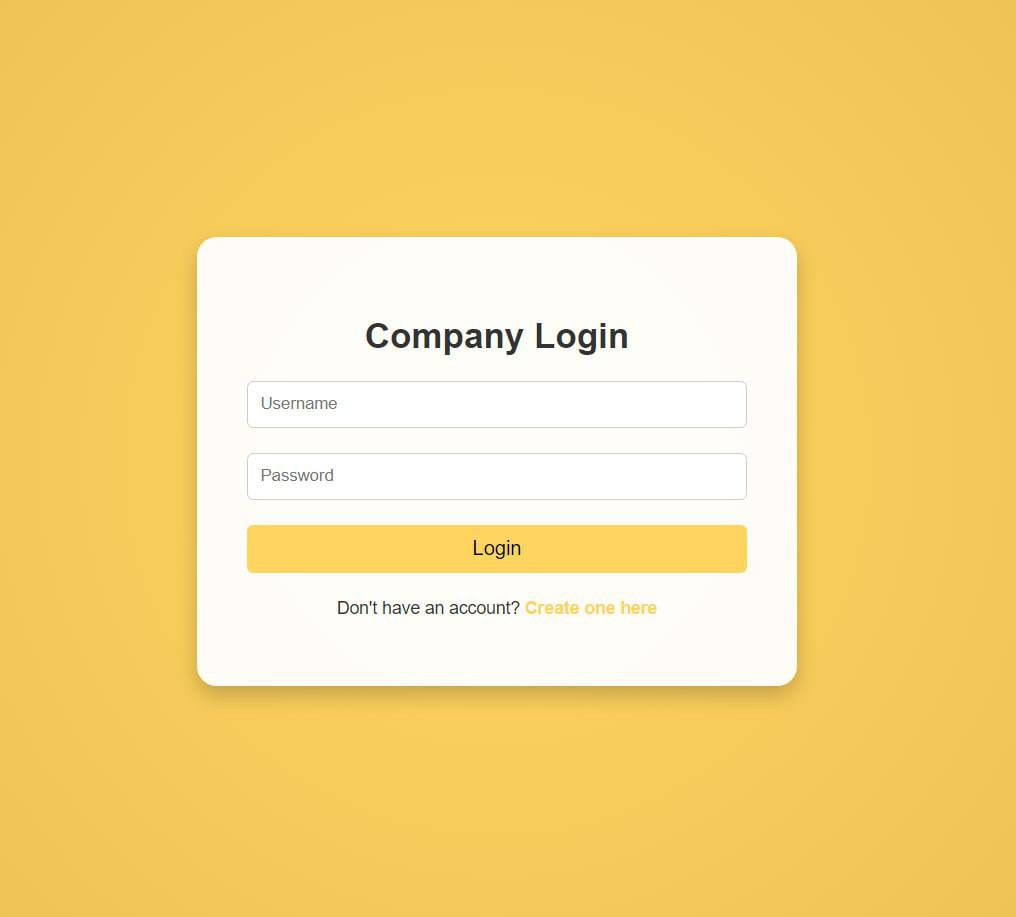
\includegraphics[width=0.8\textwidth]{Images/3.jpg}
\caption{\label{fig:metamodel3}Company Login Interface: A dedicated login form for companies to access the platform, with fields for username and password and an option for account creation.}
\end{figure}

\begin{figure}[H]
\centering
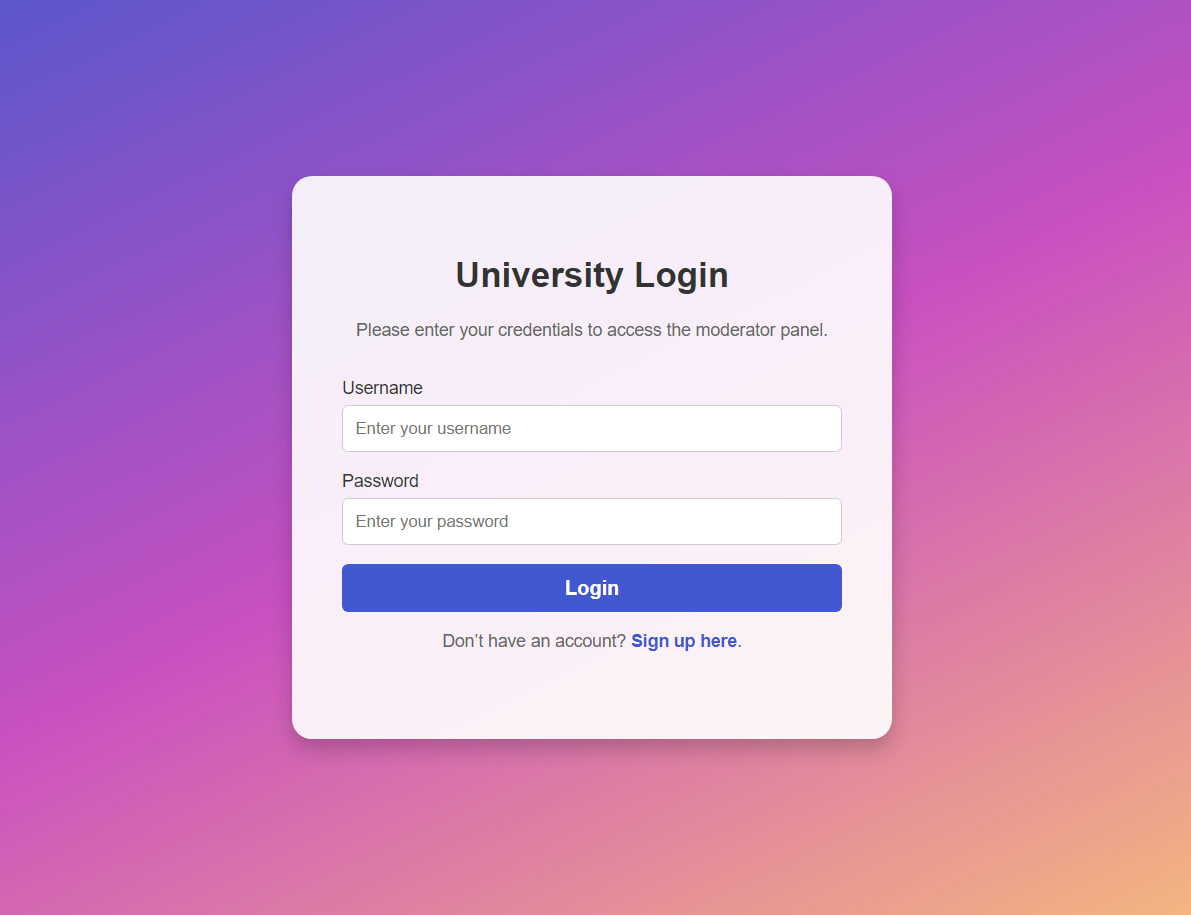
\includegraphics[width=0.8\textwidth]{Images/4.jpg}
\caption{\label{fig:metamodel4}University Login Interface: A secure login form for university moderators to access the platform, featuring fields for username and password with an option for account registration.}
\end{figure}

\begin{figure}[H]
\centering
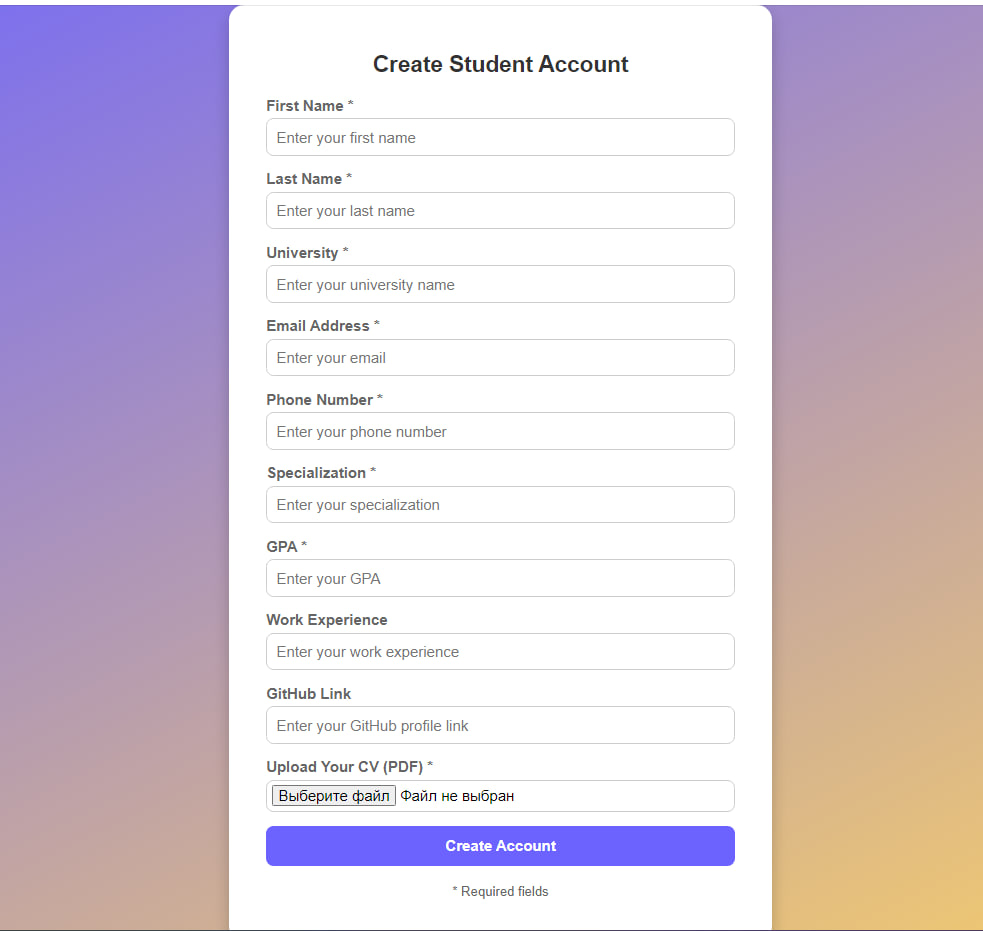
\includegraphics[width=0.8\textwidth]{Images/5.jpg}
\caption{\label{fig:metamodel5}Student Registration Form: A detailed form for students to create an account on the platform by providing personal, academic, and professional details, including uploading their CV.}
\end{figure}

\begin{figure}[H]
\centering
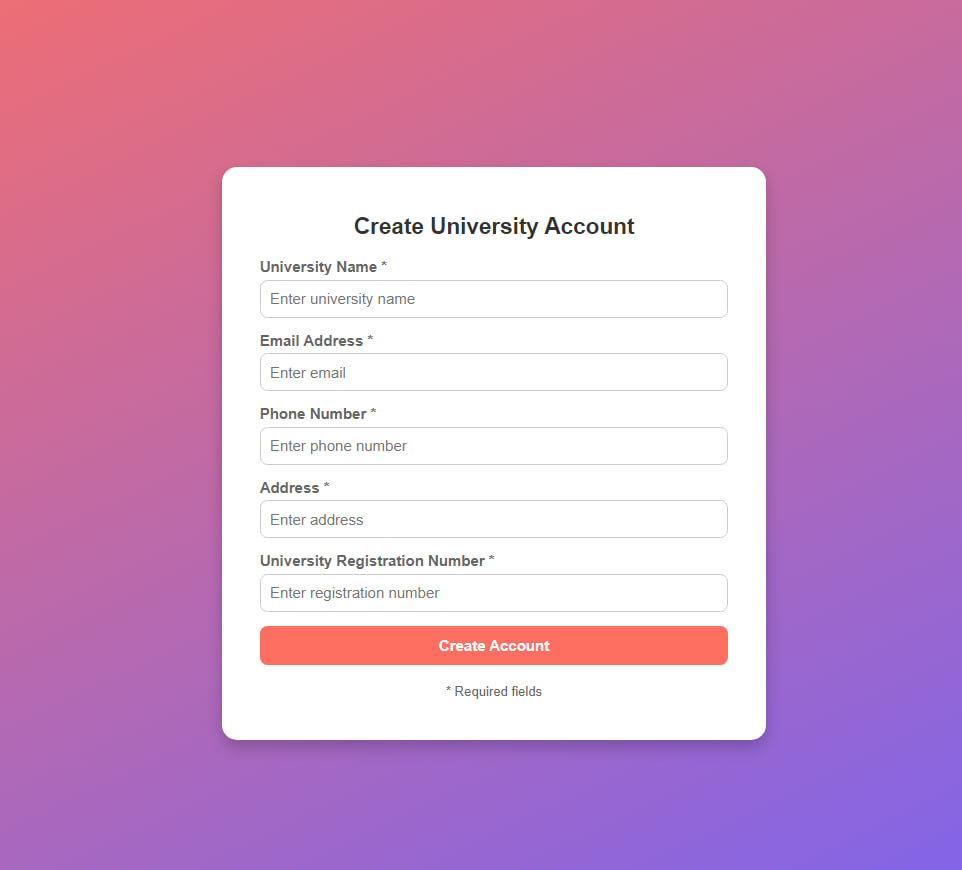
\includegraphics[width=0.8\textwidth]{Images/6.jpg}
\caption{\label{fig:metamodel6}University Registration Form: A form for universities to create an account on the platform by providing essential details such as name, email, phone number, address, and registration number.}
\end{figure}

\begin{figure}[H]
\centering
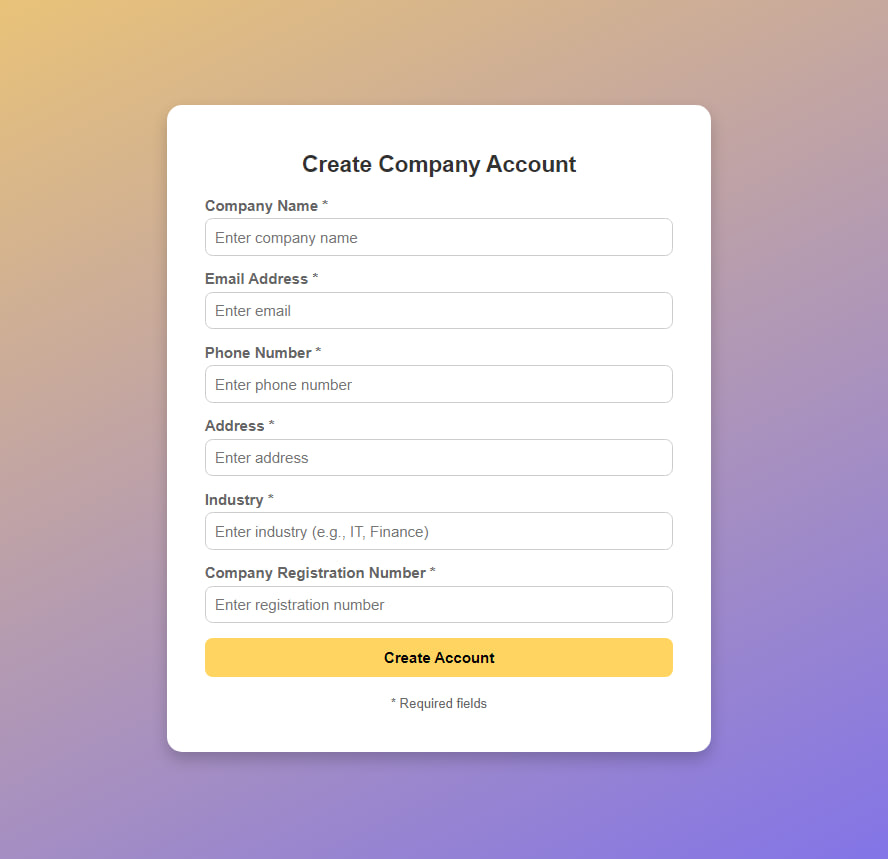
\includegraphics[width=0.8\textwidth]{Images/7.jpg}
\caption{\label{fig:metamodel7}Company Registration Form: A form for companies to create an account on the platform by providing details such as name, email, phone number, address, industry, and registration number.}
\end{figure}

\begin{figure}[H]
\centering
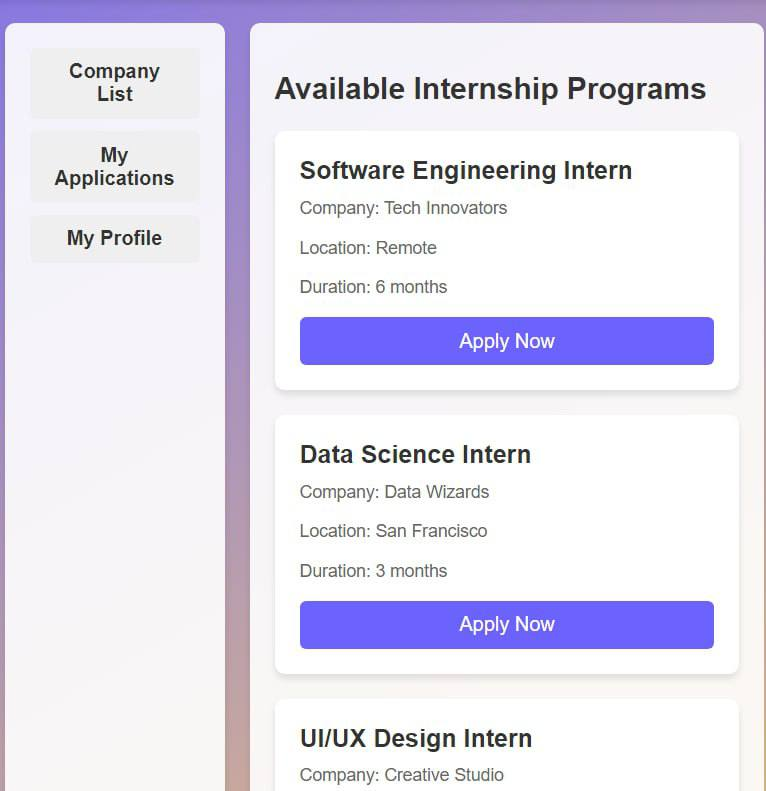
\includegraphics[width=0.8\textwidth]{Images/8.jpg}
\caption{\label{fig:metamodel8}Available Internship Programs: A user interface showcasing a list of internship opportunities with details such as position, company, location, and duration, along with an option to apply directly.}
\end{figure}

\begin{figure}[H]
\centering
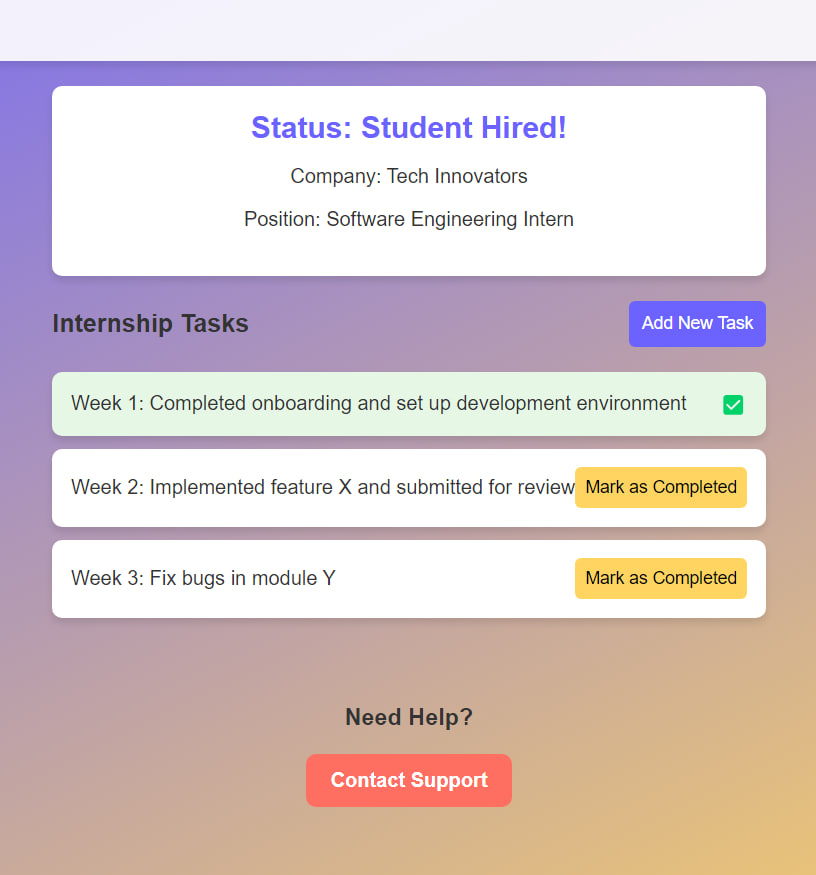
\includegraphics[width=0.8\textwidth]{Images/9.jpg}
\caption{\label{fig:metamodel9}Internship Progress Dashboard: A detailed interface for tracking the progress of assigned internship tasks, with options to mark tasks as completed and add new tasks, along with a support contact feature, in which they can address their complaints.}
\end{figure}

\begin{figure}[H]
\centering
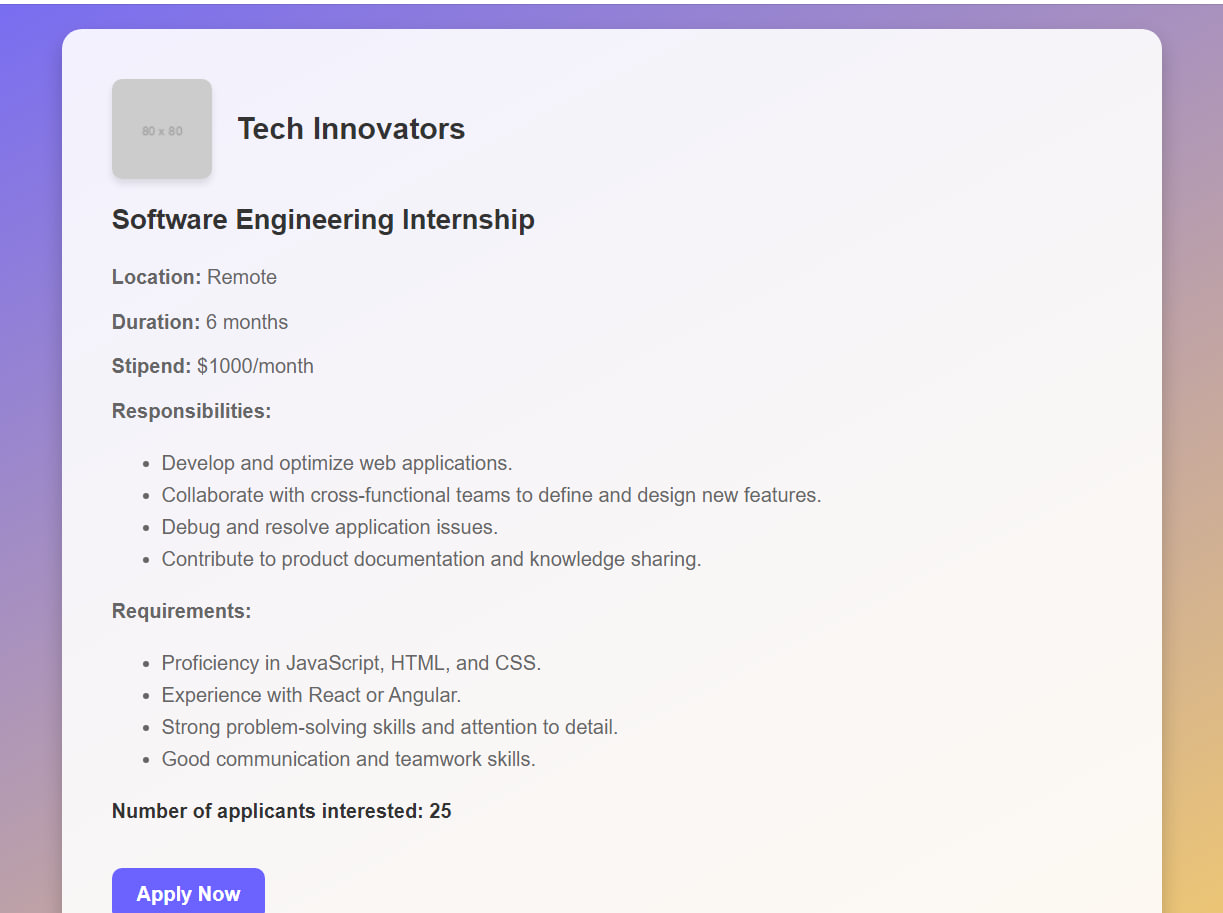
\includegraphics[width=0.8\textwidth]{Images/10.jpg}
\caption{\label{fig:metamodel10}Internship Details Page: A detailed view of an internship posting, including position, location, duration, stipend, responsibilities, and requirements, with an option to apply directly.}
\end{figure}

\begin{figure}[H]
\centering
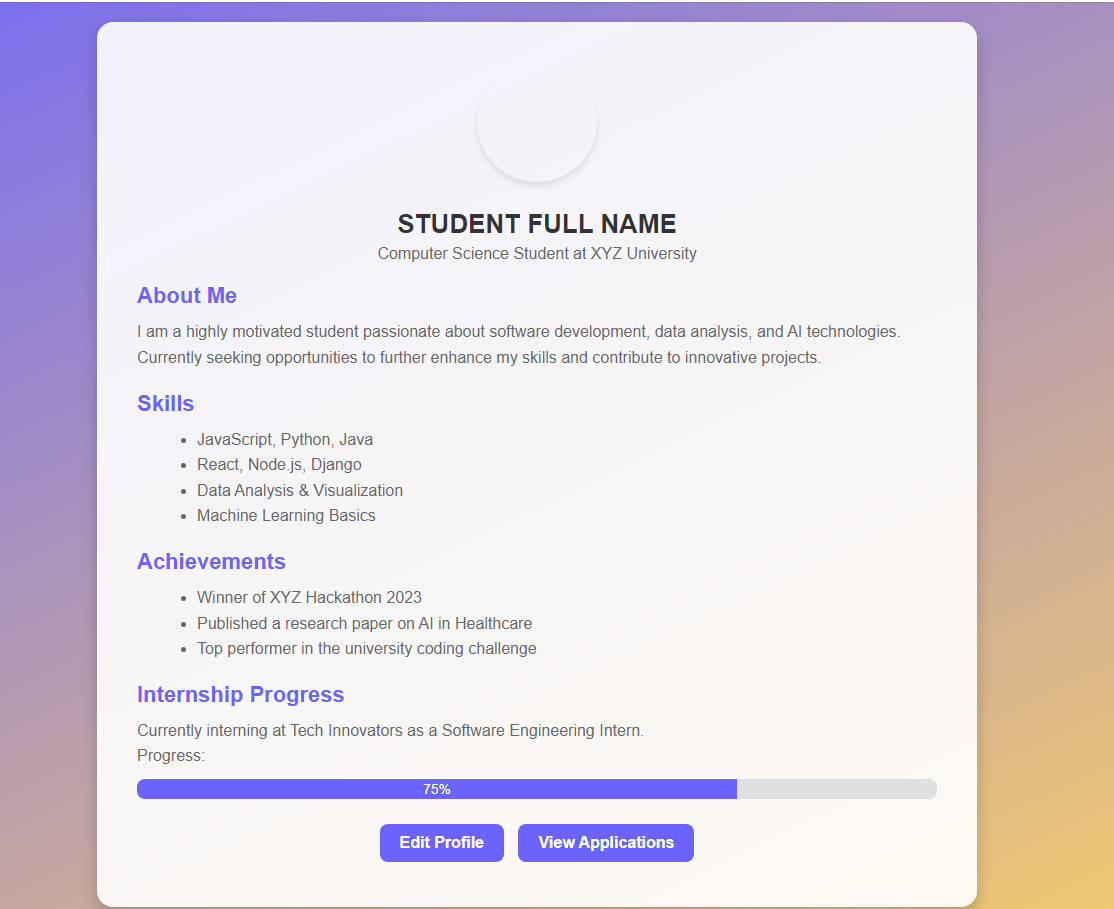
\includegraphics[width=0.8\textwidth]{Images/11.jpg}
\caption{\label{fig:metamodel11}Student Profile Page: A comprehensive profile interface displaying the student's personal information, skills, achievements, and internship progress, with options to edit the profile and view applications.}
\end{figure}

\begin{figure}[H]
\centering
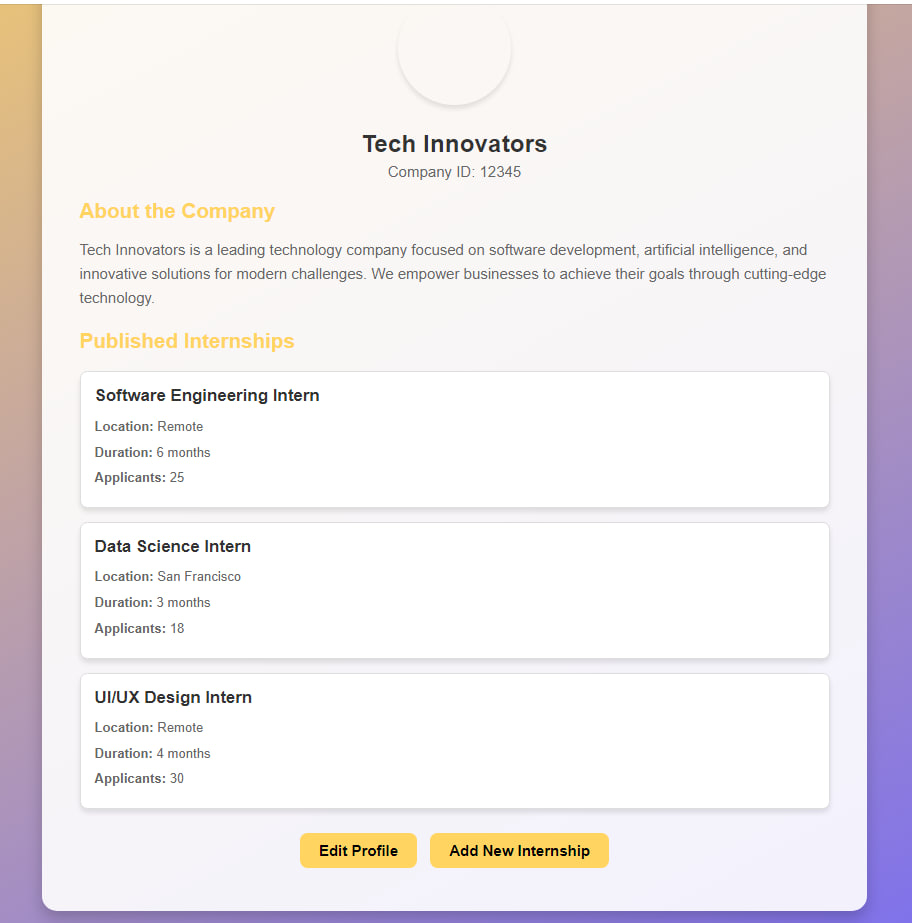
\includegraphics[width=0.8\textwidth]{Images/12.jpg}
\caption{\label{fig:metamodel12}Company Profile Page: An interface displaying the company's details, including an about section, a list of published internships with applicant information, and options to edit the profile or add new internships.}
\end{figure}

\begin{figure}[H]
\centering
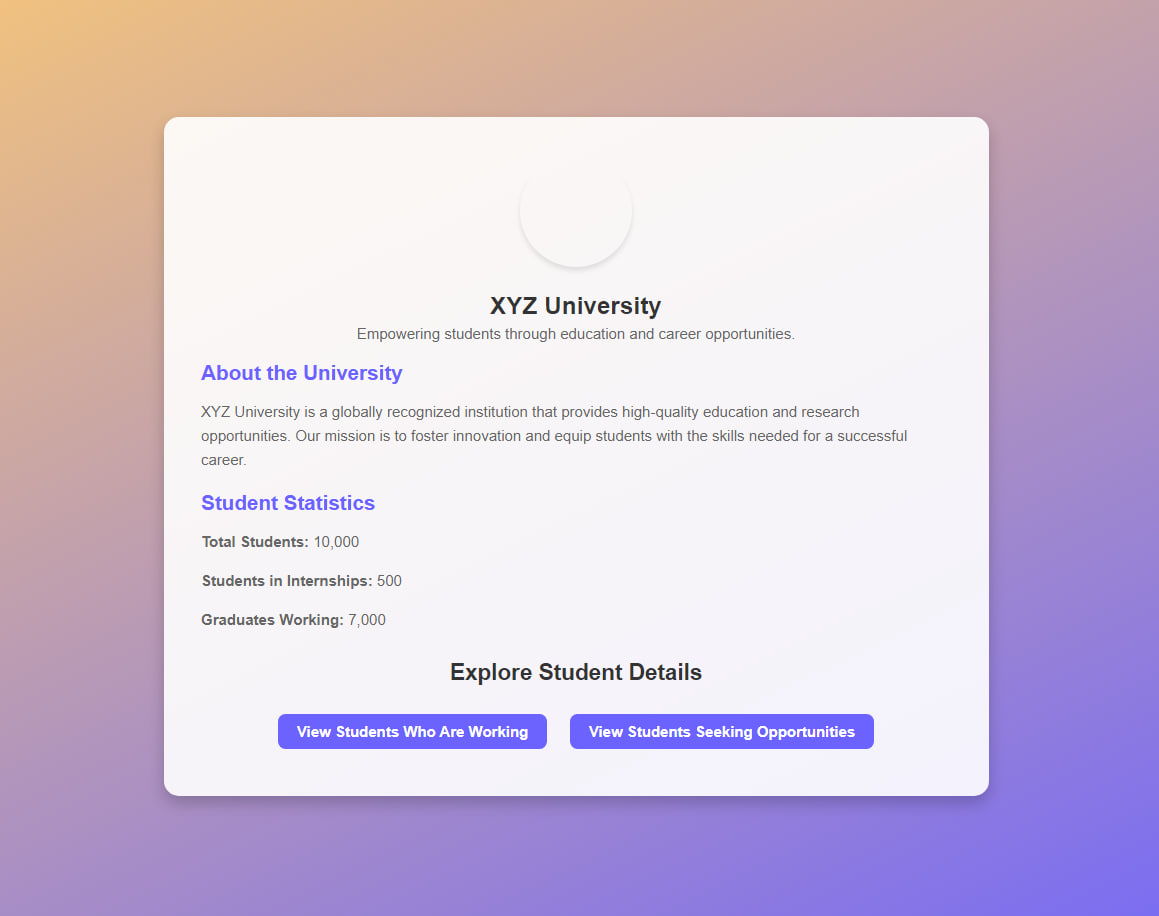
\includegraphics[width=0.8\textwidth]{Images/13.jpg}
\caption{\label{fig:metamodel13}University Profile Page: An interface displaying university details, including an about section, student statistics, and options to explore details of students who are working or seeking opportunities.}
\end{figure}


\subsubsection{Hardware Interfaces}

To interact with the Students\&Companies (S\&C) platform, all users, including students, companies, and universities, must utilize suitable devices that support internet connectivity and web browsers. The system is designed to function on standard computing devices, such as personal computers, laptops, and tablets.

These requirements ensure smooth operation of the platform, especially during real-time activities such as interviews, feedback submissions, and monitoring processes.

\subsubsection{Software Interfaces}

The Students\&Companies (S\&C) platform includes several key software components: an in-app notification system keeps users informed about important events, like new internship postings or updates to their applications. An EmailService helps with registration and sends timely updates and confirmations. The RecommendationEngine matches students with internships by analyzing their profiles and preferences. A FeedbackSystem allows users to share their thoughts, improving the platform over time. Universities can also monitor and manage internships using built-in support and complaint-handling tools.

\subsubsection{Communication Interfaces}

The Students\&Companies (S\&C) platform requires a stable internet connection to function effectively. It enables students to browse internships, companies to post opportunities, and universities to monitor ongoing internships. Reliable communication is essential for real-time notifications, updates, and interactions between all parties involved.

\subsection{Functional Requirements}
In this section, we present Use Case Diagrams and all the corresponding Use Cases. Then, the mapping between Goals, Domain Assumptions and Requirements is provided.
% \textbf{Sign up and log in}\\
% \texttt{[R1]} The system allows users (students, companies, and universities) to register by providing their personal information (e.g., name, email address, and password). \\
% \texttt{[R2]} The system allows registered users to log in and manage their accounts. \\
% \texttt{[R3]} The system enables users to update their profile information when necessary. \\

% \textbf{Internship Management}\\
% \texttt{[R4]} Companies can create, modify, and delete internship postings by specifying details such as title, description, required skills, technologies, and benefits. \\
% \texttt{[R5]} Companies can track applications and review candidate CVs associated with their internships. \\
% \texttt{[R6]} Companies can schedule interviews and send notifications to students regarding their status. \\
% \texttt{[R7]} Companies can provide feedback and suggestions for improving student submissions. \\
% \texttt{[R8]} Companies can monitor and evaluate students' progress during internships by assigning and tracking tasks.\\

% \textbf{Student Interaction}\\
% \texttt{[R9]} Students can search and apply for internships. \\
% \texttt{[R10]} Students can receive personalized recommendations for internships based on their profiles, skills, and preferences. \\
% \texttt{[R11]} Students can update and maintain their CVs and submit them for applications. \\
% \texttt{[R12]} Students can provide feedback about internships and companies. \\
% \texttt{[R13]} Students can file complaints if issues arise during an internship. \\

% \textbf{University Monitoring}\\
% \texttt{[R14]} Universities can monitor the status of internships undertaken by their students. \\
% \texttt{[R15]} Universities can handle complaints and resolve issues reported by students or companies. \\
% \texttt{[R16]} Universities can track the overall performance of students during internships and maintain records for future analysis. \\

% \textbf{Recommendation and Feedback System}\\
% \texttt{[R17]} The system uses a recommendation engine to match students with internships based on skills, preferences. \\
% \texttt{[R18]} The system collects and analyzes feedback from students and companies to improve the recommendation accuracy. \\

% \textbf{Communication and Notification}\\
% \texttt{[R19]} The system sends notifications to users about updates, deadlines, and interview schedules. \\
% \texttt{[R20]} The system alerts users about any issues or conflicts that require their attention. \\

\subsubsection{Use Case Diagrams}

\begin{figure}[H]
\centering
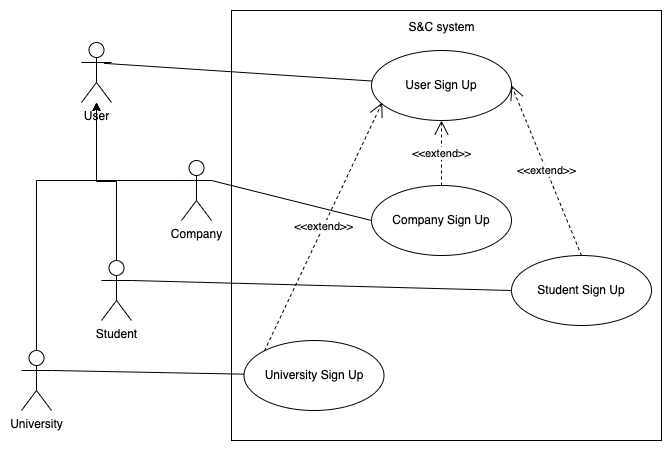
\includegraphics[width=0.8\textwidth]{Images/SignUP_Use_Case_Diagram.png}
\caption{\label{fig:metamodel9}Sign Up Use Case Diagram.}
\end{figure}

\begin{figure}[H]
\centering
\includegraphics[width=0.8\textwidth]
%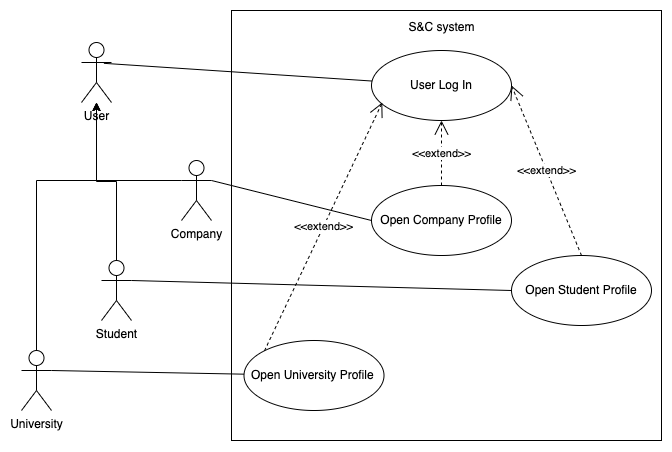
\includegraphics[scale=0.20]
{Images/Log_In_Use_Case_Diagram.png}
\caption{\label{fig:metamodel9}Log In Use Case Diagram.}
\end{figure}


\begin{figure}[H]
\centering
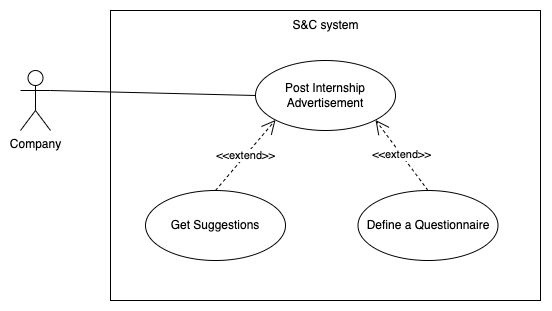
\includegraphics[width=0.8\textwidth]{Images/Internship_Adding_Use_Case_Diagram.png}
\caption{\label{fig:metamodel9}Posting Internship Advertisement Use Case Diagram.}
\end{figure}


\begin{figure}[H]
\centering
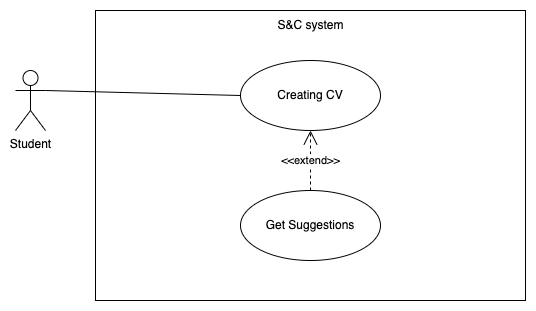
\includegraphics[width=0.8\textwidth]{Images/CV_Creation_Use_Case_Diagram.png}
\caption{\label{fig:metamodel9}CV Creation Use Case Diagram.}
\end{figure}


\begin{figure}[H]
\centering
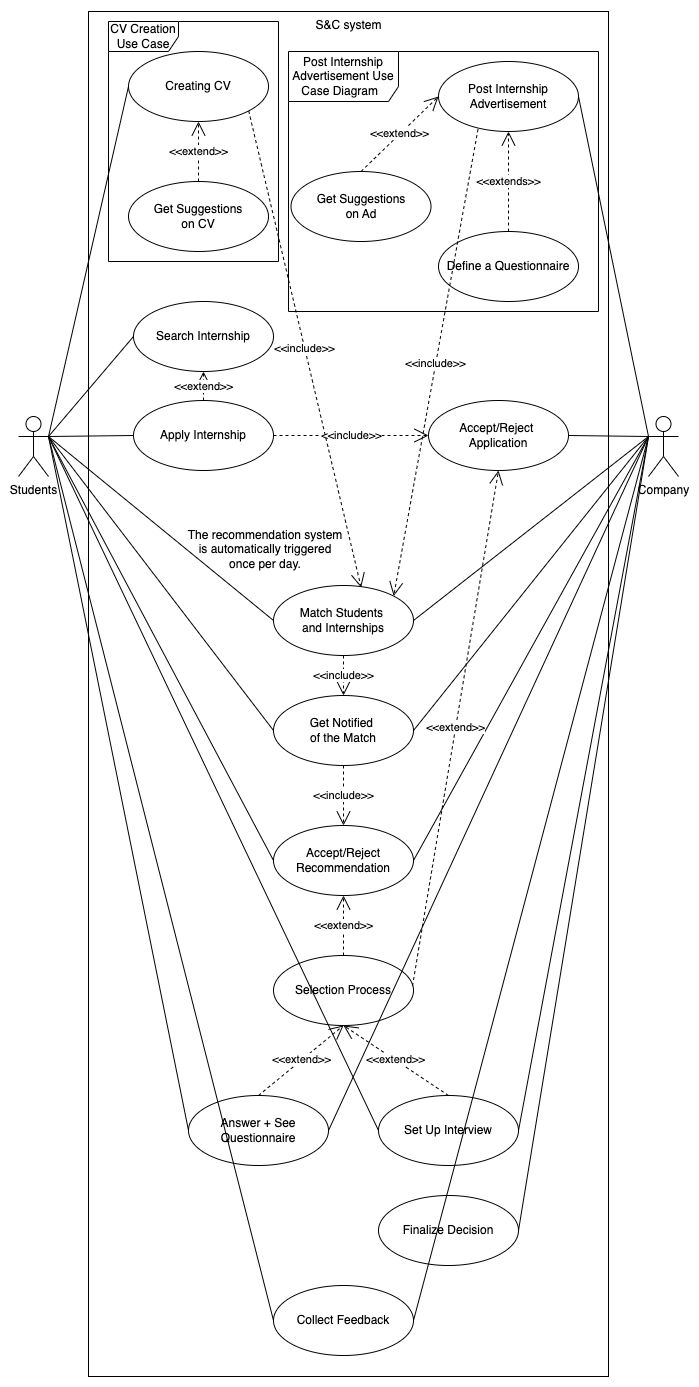
\includegraphics[width=0.8\textwidth]{Images/Main_Use_Case_Diagram.png}
\caption{\label{fig:metamodel9}Main Use Case Diagram.}
\end{figure}

\begin{figure}[H]
\centering
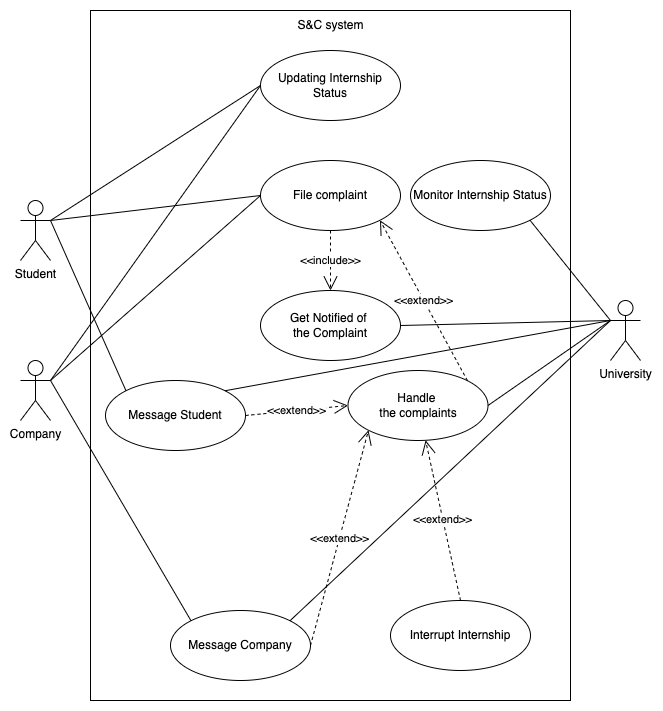
\includegraphics[width=0.8\textwidth]{Images/Complaint_handling_Use_Case_Diagram.png}
\caption{\label{fig:metamodel9}Complaint and Internship Status Use Case Diagram.}
\end{figure}

\subsubsection{Use Cases}

In this section we discuss the most important use cases from the diagrams.

\begin{table}[H]
\centering
\begin{tabular}{|l|p{12cm}|}
\hline
Name             & User Sign Up \\ \hline
Actor            & User (General) \\ \hline
Entry Condition  & 
The user accesses the S\&C system and selects the sign-up option. The user has not already registered in the system. \\ \hline
Event flow       & 
\begin{enumerate}
    \item User opens the sign-up page.
    \item User fills in basic information (e.g., name, email, password).
    \item User selects the type of account (Company, Student, or University).
    \item System validates the input.
    \item User account is created.
\end{enumerate} \\ \hline
Exit Condition   & The user successfully registers and can log in to the system. \\ \hline
Exception        & 
\begin{enumerate}
    \item Input validation fails (e.g., invalid email or password criteria not met).
\item User already has an account.
\end{enumerate} \\ \hline
Special Reqs     & The system must ensure data security during registration. An email verification process may be required. \\ \hline
Inheritance Relationship & 
\begin{itemize}
    \item Company Sign Up: Extends User Sign Up with additional fields for company details (e.g., registration number).
    \item Student Sign Up: Extends User Sign Up with fields for educational details (e.g., student ID, degree program).
    \item University Sign Up: Extends User Sign Up with institutional details (e.g., university name, accreditation). 
\end{itemize} \\ \hline
\end{tabular}
\caption{Use Case 1: User Sign Up}
\label{tab:user_signup}
\end{table}

\begin{table}[H]
\centering
\begin{tabular}{|l|p{12cm}|}
\hline
Name             & User Log In \\ \hline
Actor            & User (General) \\ \hline
Entry Condition  & 
The user accesses the S\&C system and navigates to the log-in page. The user already has a registered account. \\ \hline
Event flow       & 
\begin{enumerate}
    \item User opens the log-in page.
    \item User enters their credentials (e.g., email and password).
    \item System validates the credentials.
    \item Upon successful validation, the system directs the user to their respective profile page (Company, Student, or University).
\end{enumerate} \\ \hline
Exit Condition   & The user successfully logs in and accesses their account dashboard. \\ \hline
Exception        & 
\begin{enumerate}
    \item Invalid credentials (e.g., incorrect email or password).
    \item User account is not found in the database.
\end{enumerate} \\ \hline
Special Reqs     & The system must securely encrypt the user credentials during transmission and ensure compliance with data protection standards. \\ \hline
Inheritance Relationship & 
\begin{itemize}
    \item Company Log In: Redirects to the Company Profile upon successful authentication.
    \item Student Log In: Redirects to the Student Profile upon successful authentication.
    \item University Log In: Redirects to the University Profile upon successful authentication. 
\end{itemize} \\ \hline
\end{tabular}
\caption{Use Case 2: User Log In}
\label{tab:user_login}
\end{table}

\begin{table}[H]
\centering
\begin{tabular}{|l|p{12cm}|}
\hline
Name             & Creating CV \\ \hline
Actor            & Student \\ \hline
Entry Condition  & 
The student logs into the system and selects the "Create CV" option. \\ \hline
Event Flow       & 
\begin{enumerate}
    \item User accesses the "Create CV" page.
    \item User enters personal details, educational background, work experience, skills, certifications, soft skills, and other relevant information.
    \item System auto-formats the provided details into a CV using a predefined template.
    \item System automatically triggers the "Get Suggestions on CV" use case to evaluate the CV and provide feedback.
\end{enumerate} \\ \hline
Exit Condition   & 
The CV is successfully created, and the user can view, download, or Edit it. \\ \hline
Exception        & 
\begin{enumerate}
    \item Missing or invalid data entered by the user (e.g., empty mandatory fields like name or email).
    \item System encounters formatting errors while generating the CV.
\end{enumerate} \\ \hline
Special Reqs     & 
The system must ensure seamless CV generation and provide a user-friendly interface for entering details. \\ \hline
Includes        & 
\begin{itemize}
    \item Get Suggestions on CV: The System automatically evaluates and provides feedback on the created CV. 
\end{itemize} \\ \hline
\end{tabular}
\caption{Use Case 3: Creating CV}
\label{tab:create_cv}
\end{table}

\begin{table}[H]
\centering
\begin{tabular}{|l|p{12cm}|}
\hline
Name             & Get Suggestions on CV \\ \hline
Actor            & System (AI module, triggered by the "Creating CV" use case) \\ \hline
Entry Condition  & 
The "Creating CV" use case is completed, and the system has generated a formatted CV. \\ \hline
Event Flow       & 
\begin{enumerate}
    \item System receives the formatted CV from the "Creating CV" use case.
    \item AI module analyzes the CV based on predefined criteria, such as:
    \begin{itemize}
        \item Grammar and spelling accuracy.
        \item CV structure and formatting.
        \item Relevance and quality of content (e.g., measurable achievements in work experience).
        \item Suggestions tailored to the user's industry or role.
    \end{itemize}
    \item AI generates actionable, section-specific feedback (e.g., "Use bullet points to highlight key skills in the Skills section").
    \item System displays the AI-generated suggestions to the user in the "Creating CV" interface.
\end{enumerate} \\ \hline
Exit Condition   & 
The AI provides clear and actionable suggestions for improvement, and the user can revise their CV accordingly. \\ \hline
Exception        & 
\begin{enumerate}
    \item AI module fails to analyze the CV due to parsing or formatting issues.
    \item Feedback is incomplete or generic due to insufficient CV content.
\end{enumerate} \\ \hline
Special Reqs     & 
\begin{itemize}
    \item The AI must use reliable natural language processing (NLP) models for analysis.
    \item The AI model can be also interactive and take into account the user's preferences.
\end{itemize} \\ \hline
\end{tabular}
\caption{Use Case 4: Get Suggestions (AI-Powered)}
\label{tab:get_suggestions}
\end{table}

\begin{table}[H]
\centering
\begin{tabular}{|l|p{12cm}|}
\hline
Name             & Post Internship Advertisement \\ \hline
Actor            & Company \\ \hline
Entry Condition  & The company logs into the system and selects the "Post Internship Advertisement" option. \\ \hline
Event Flow       & 
\begin{enumerate}
    \item Company accesses the "Post Internship Advertisement" page.
    \item Company enters details such as:
    \begin{itemize}
        \item Internship conditions (e.g., eligibility criteria, duration, location).
        \item Project information (e.g., application domain, tasks to be performed, adopted technologies).
        \item Terms offered (e.g., paid internships, benefits like mentorship, training, etc.).
    \end{itemize}
    \item System validates the provided information.
    \item System saves the internship advertisement.
    \item System automatically triggers the AI-powered "Get Suggestions on Ad" and "Match Students and Internships" use cases.
    \item Company can decide to extend the advertisement by creating a questionnaire for applicants ("Define a Questionnaire").
\end{enumerate} \\ \hline
Exit Condition   & The internship advertisement is successfully posted, and related use cases are triggered. \\ \hline
Exception        & 
\begin{enumerate}
    \item Invalid or incomplete input from the company (e.g., missing mandatory fields).
    \item System error in saving the advertisement or triggering subsequent processes.
\end{enumerate} \\ \hline
Special Reqs     & 
\begin{enumerate}
    \item The system must provide an intuitive interface for entering advertisement details.
    \item The system should ensure data security and privacy.
\end{enumerate} \\ \hline
Includes         & 
\begin{itemize}
    \item Get Suggestions on Ad: Automatically analyzes and provides feedback on the advertisement using AI.
    \item Match Students and Internships: Automatically matches posted internships with suitable students based on their profiles and preferences.
\end{itemize} \\ \hline
Extended by          & 
\begin{itemize}
    \item Define a Questionnaire: Companies can add a custom questionnaire for applicants after posting the advertisement.
\end{itemize} \\ \hline
\end{tabular}
\caption{Use Case 5: Post Internship Advertisement}
\label{tab:post_internship}
\end{table}

\begin{table}[H]
\centering
\begin{tabular}{|l|p{12cm}|}
\hline
Name             & Get Suggestions on Ad \\ \hline
Actor            & System (AI module) \\ \hline
Entry Condition  & The "Post Internship Advertisement" use case is completed, and the advertisement details are saved. \\ \hline
Event Flow       & 
\begin{enumerate}
    \item System (AI module) analyzes the posted advertisement based on:
    \begin{itemize}
        \item Completeness and clarity of details.
        \item Alignment with common standards for internships.
        \item Potential industry-specific improvements.
    \end{itemize}
    \item AI suggests:
    \begin{itemize}
        \item Revisions to improve clarity or attractiveness of the advertisement.
        \item Additional details to enhance applicant understanding (e.g., elaboration on benefits or tasks).
    \end{itemize}
    \item Suggestions are interactive, allowing the company to provide preferences or constraints.
    \item Company can choose to make the changes suggested by the AI model or not.
\end{enumerate} \\ \hline
Exit Condition   & The company receives actionable, AI-generated suggestions for improving the advertisement. \\ \hline
Exception        & 
\begin{enumerate}
    \item AI module fails to analyze due to missing or poorly formatted input.
    \item Suggestions fail to reflect relevant industry standards due to insufficient training of the AI. 
\end{enumerate} \\ \hline
Special Reqs     & 
\begin{enumerate}
    \item The AI module must use reliable NLP and domain-specific models.
    \item Feedback must be clear, actionable, and aligned with the company's preferences.
\end{enumerate} \\ \hline
Included By      & 
\begin{itemize}
    \item \textbf{Post Internship Advertisement:} Automatically triggers this use case upon posting the advertisement.
\end{itemize} \\ \hline
\end{tabular}
\caption{Use Case 6: Get Suggestions on Ad}
\label{tab:get_suggestions_ad}
\end{table}

\begin{table}[H]
\centering
\begin{tabular}{|l|p{12cm}|}
\hline
Name             & Define a Questionnaire \\ \hline
Actor            & Company \\ \hline
Entry Condition  & 
The "Post Internship Advertisement" use case is completed, and the company has decided to create a questionnaire for applicants. \\ \hline
Event Flow       & 
\begin{enumerate}
    \item Company selects the "Define a Questionnaire" option for a specific internship advertisement.
    \item Company creates a questionnaire by:
    \begin{itemize}
        \item Adding questions relevant to the internship role (e.g., technical knowledge, situational questions).
        \item Choosing question types (e.g., multiple-choice, open-ended, rating scale).
        \item Setting criteria for evaluation, such as scoring weightage or mandatory responses.
    \end{itemize}
    \item System validates the questionnaire for completeness (e.g., no missing question fields, proper format).
    \item System saves the questionnaire and links it to the corresponding internship advertisement.
    \item Company can edit or update the questionnaire before publishing it for applicants. 
\end{enumerate} \\ \hline
Exit Condition   & 
The questionnaire is successfully created, validated, and linked to the internship advertisement for applicant use. \\ \hline
Exception        & 
\begin{enumerate}
    \item Company provides incomplete or invalid inputs (e.g., missing question text, improper formats).
    \item System encounters errors while saving or linking the questionnaire to the advertisement.
\end{enumerate} \\ \hline
Special Reqs     & 
\begin{enumerate}
    \item The system must allow easy customization of questionnaires, including different question types and evaluation criteria.
    \item The system should validate and ensure completeness and consistency of the questionnaire.
    \item Questionnaires must be securely saved and accessible only to authorized users (company and relevant applicants).
\end{enumerate} \\ \hline
Extends          & 
\begin{itemize}
    \item Post Internship Advertisement: Extends this use case by enabling additional applicant evaluation functionality.
\end{itemize} \\ \hline
\end{tabular}
\caption{Use Case 7: Define a Questionnaire}
\label{tab:define_questionnaire}
\end{table}

\begin{table}[H]
\centering
\begin{tabular}{|l|p{12cm}|}
\hline
Name             & Search Internship \\ \hline
Actor            & Student \\ \hline
Entry Condition  & The student logs into the system and selects the "Search Internship" option. \\ \hline
Event Flow       & 
\begin{enumerate}
    \item Student accesses the "Search Internship" module.
    \item Student enters search criteria, such as:
    \begin{itemize}
        \item Skills and qualifications.
        \item Location preferences.
        \item Internship type (e.g., paid, remote).
    \end{itemize}
    \item System retrieves and displays a list of internships matching the criteria.
    \item Student reviews the results and selects an internship for further details.
    \item If the student finds a suitable internship, they can proceed to "Apply Internship."
\end{enumerate} \\ \hline
Exit Condition   & 
The student either reviews a list of matching internships or proceeds to apply for a specific one. \\ \hline
Exception        & 
\begin{enumerate}
    \item No internships match the provided criteria.
    \item System error in retrieving or displaying internship details.
\end{enumerate} \\ \hline
Special Reqs     & 
\begin{enumerate}
    \item The system must allow filtering and sorting of search results.
    \item The system should ensure real-time updates on available internships.
\end{enumerate} \\ \hline
Extended by          & 
\begin{itemize}
    \item Apply Internship: Extends this use case if the student chooses to apply for an internship.
\end{itemize} \\ \hline
\end{tabular}
\caption{Use Case 8: Search Internship}
\label{tab:search_internship}
\end{table}

\begin{table}[H]
\centering
\begin{tabular}{|l|p{12cm}|}
\hline
Name             & Apply Internship \\ \hline
Actor            & Student \\ \hline
Entry Condition  & 
The student finds a suitable internship during the "Search Internship" use case and decides to apply. \\ \hline
Event Flow       & 
\begin{enumerate}
    \item Student selects the "Apply" option for a specific internship.
    \item System prompts the student to upload or confirm their application materials (e.g., CV, cover letter).
    \item System validates the completeness of the application.
    \item System submits the application and notifies the corresponding company.
\end{enumerate} \\ \hline
Exit Condition   & 
The student's application is successfully submitted to the company for review. \\ \hline
Exception        & 
\begin{enumerate}
    \item Application materials are incomplete or invalid.
    \item System encounters an error in submitting the application.
\end{enumerate} \\ \hline
Special Reqs     & 
Notifications must be sent to the company upon successful submission. \\ \hline
Extends      & 
\begin{itemize}
    \item \textbf{Search Internship:} This use case is triggered when a student decides to apply for an internship found during the search.
\end{itemize} \\ \hline
Includes         & 
\begin{itemize}
    \item \textbf{Accept/Reject Application:} Automatically triggers this use case for the company after submission.
\end{itemize} \\ \hline
\end{tabular}
\caption{Use Case 9: Apply Internship}
\label{tab:apply_internship}
\end{table}

\begin{table}[H]
\centering
\begin{tabular}{|l|p{12cm}|}
\hline
Name             & Accept/Reject Application \\ \hline
Actor            & Company \\ \hline
Entry Condition  & 
The company receives a notification that a student has applied for an internship. \\ \hline
Event Flow       & 
\begin{enumerate}
    \item Company accesses the "Accept/Reject Application" module from the sent notification.
    \item Company reviews the student's application materials (e.g., CV, cover letter).
    \item Company evaluates the application based on their initial criteria.
    \item Company either:
    \begin{itemize}
        \item Accepts the application, triggering the "Selection Process" use case.
        \item Rejects the application, sending a notification to the student.
    \end{itemize}
\end{enumerate} \\ \hline
Exit Condition   & 
The company either accepts or rejects the application, and the corresponding actions are triggered. \\ \hline
Exception        & 
\begin{enumerate}
    \item Application materials are incomplete or corrupted.
    \item System error in notifying the company or processing the decision.
\end{enumerate} \\ \hline
Special Reqs     & 
\begin{enumerate}
    \item Notifications must be sent to the student upon decision.
    \item The system must ensure secure access to application materials.
\end{enumerate} \\ \hline
Included By      & 
\begin{itemize}
    \item Apply Internship: Automatically triggers this use case when a student submits an application.
\end{itemize} \\ \hline
Includes         & 
\begin{itemize}
    \item Selection Process: Automatically triggered when an application is accepted.
\end{itemize} \\ \hline
\end{tabular}
\caption{Use Case 10: Accept/Reject Application}
\label{tab:accept_reject_application}
\end{table}




\begin{table}[H]
    \centering
    \begin{tabular}{|l|p{12cm}|}
    \hline
    Name             & Match Students and Internships \\ \hline
    Actor            & Student, Company \\ \hline
    Entry Condition  & 
    The profile of the student and job listing by the company is available \\ \hline
    Event flow       & 
    \begin{enumerate}
        \item Students have uploaded provife and created CV.
        \item Companies have posted internship roles.
        \item S\&C gathers available student information and internship listings
        \item S\&C applies matching algorithm based on student details and internship requirements like technical skills, soft skills, experience needed, grades.
        \item S\&C platform identifies company and student matches based on highest recommendation percentage.
        \item Both matched student and company are then notified and the recommendation is shown in respective dashboards.
        \item Both parties then can accept or reject the project by clicking the respective buttons. 
    \end{enumerate} \\ \hline
    Exit Condition   & Recommendations shown and notified to students and companies \\ \hline
    Exception        & 
    \begin{enumerate}
        \item No matches are found.
    \item The system waits for new or changes in profiles or listings.
\end{enumerate} \\ \hline
Special Reqs     & The system must ensure accurate analysis of data for correct and meaningful results. A notification provider may be required. \\ \hline
\end{tabular}
\caption{Use Case 11: Match Students and Internships}
\label{tab:user_signup}
\end{table}


\begin{table}[H]
    \centering
    \begin{tabular}{|l|p{12cm}|}
    \hline
    Name             & Selection Process \\ \hline
    Actor            & Student, Company \\ \hline
    Entry Condition  & 
    \begin{enumerate}
        \item The student has applied for the internship and has been selected to go through more evaluations.
        \item The student and company both have accepted the systems recommendation to match.
    \end{enumerate} \\ \hline
    Event flow       & 
    \begin{enumerate}
        \item The system opens a communication channel between the student and company.
        \item The system notify both the student and the company that the selection process for that specific internship has started and now then can contact each other. 
        \item If a questionnaire is already created for the internship, the system shows that to the student and prompt them to fill the questionnaire out.
        \item If a questionnaire is not already created by the company, the system sends a notification to them to remind them that they still can create a questionnaire from the internship dashboard.
        \item After the student submits the answers to the questionnaire, the company is notified instantly. 
        \item The company then reviews the answers by the student and accordingly decides to interview or not by clicking on "Select for Interview" or "Reject" buttons.
        \item A notification is sent to the student instantly.
        \item If selected, the student is added to the list of students shortlisted for interview for that role.
        \item The system initiates the "Set Up Interview" process. 
    \end{enumerate} \\ \hline
    Exit Condition   & Student is selected for an interview \\ \hline
    Exception        & 
    \begin{enumerate}
        \item Technical issues prevent the communication channel from initializing.
        \item The student fails to complete the questionnaire before the deadline.
        \item The student is unreachable and does not respond to notifications.
        \item Notifications fail to reach either the student or the company.
\end{enumerate} \\ \hline
\end{tabular}
\caption{Use Case 12: Company finalize student for interview}
\label{tab:user_signup}
\end{table}


\begin{table}[H]
    \centering
    \begin{tabular}{|l|p{12cm}|}
    \hline
    Name             & Set Up Interview (S\&C Platform Manage Interview Process) \\ \hline
    Actor            & Student, Company \\ \hline
    Entry Condition  & 
    The selection process has started and the company has decided to take an interview from the student. \\ \hline
    Event flow       & 
    \begin{enumerate}
        \item The platform prompts the company to select available time slots for the interview from the calender system in the platform.
        \item The platform then prompts the student to select a suitable slot from the ones provided by company.
        \item The system sends a confirmation to both the student and company with the scheduled date, time, and interview format.
        \item The system generates a unique interview link (if video interview) or location (if in-person) 
        \item Notifications are sent instantly sharing the info with both the company and student.
        \item The platform sets up reminders for both parties, notifying them 24 hours and 1 hour before the interview.
        \item The interview takes place as per the scheduled time.
        % \item The system may facilitate a structured interview process by allowing the company to set up pre-configured questions or questionnaires.
        \item The system updates the status of the interview (e.g., "Scheduled," "Completed," "Pending Feedback").
        \item After the interview, the company can decide to go for a "Second Round Interview" by clicking the button or move forward to finalizing the decision on the student in the internship dashboard("Finalize Decision").

        % \item Once the interview is completed, the platform prompts both the student and company to provide feedback on the interview.
        % \item The system archives all relevant data (e.g., interview feedback, results) for future analysis or recommendations.

    \end{enumerate} \\ \hline
    Exit Condition   & 
    \begin{enumerate}
        \item The interview is set and takes place.
    \end{enumerate} \\ \hline
    Exception        & 
    \begin{enumerate}
        \item Interview link/Location not accessible.
        \item No response from company or student.
        \item Platform failure during interview.
\end{enumerate} \\ \hline
Special Reqs     & Secure Video Conferencing Integration\\ \hline
\end{tabular}
\caption{Use Case 13: Set Up Interview}
\label{tab:user_signup}
\end{table}


\begin{table}[H]
    \centering
    \begin{tabular}{|l|p{12cm}|}
    \hline
    Name             & Finalize Decision (company finalize the decision for selection process) \\ \hline
    Actor            & Student, Company \\ \hline
    Entry Condition  & 
    The company has reviewed the student profile and questionnaire's answers and is interested in recruiting the student for the internship\\ \hline
    Event flow       & 
    \begin{enumerate}
        \item Company opens the internship page. 
        \item Company clicks "show interviewed students" and reviews the list of students whom undergone interviews for the specific internship position either from applications or system match recommendations.
        \item If the company chooses to recruit a student, clicks on the "Accept" button for that student.
        \item If the company chooses to reject a student, clicks on the "Reject" button for that student.
        \item A notification is sent to the student instantly informing the student of the final decision.
        \item The system records this decision in the student's profile and updates the status of the internship application.
    \end{enumerate} \\ \hline
    Exit Condition   & The final decision on the recruitment of a student for an internship is made. \\ \hline
    Exception        & 
    \begin{enumerate}
        \item No student listed for the position.
        \item The student has already accepted another internship offer but remains on the list.
        \item The system fails to log the company's decision (accept or reject).
\end{enumerate} \\ \hline
\end{tabular}
\caption{Use Case 14: Company finalize student for interview}
\label{tab:user_signup}
\end{table}


\begin{table}[H]
    \centering
    \begin{tabular}{|l|p{12cm}|}
    \hline
    Name             & Collect Feedback \\ \hline
    Actor            & Student, Company  \\ \hline
    Entry Condition  & 
    Both the student and the company have gone through selection process and now know each other better. \\ \hline
    Event flow       & 
    \begin{enumerate}
        \item The system collects application data and also takes into account the final decision on the recommendation.
        \item The system asks both parties to fill out a "feedback form" on the match that was made between them.
        \item Students and companies rate the service by the S\&C platform between 1 to 5 stars and answer relevant questions related to the process and give suggestions on what could be better.
        \item The system analyses the collected data using statistical analysis and natural language processing.
        \item Based on the analysis the recommendation system is adjusted and improved recommendation are shown to users
    \end{enumerate} \\ \hline
    Exit Condition   & 
    \begin{enumerate}
        \item The systems recommendation system is updated based on feedback provided
        \item Future recommendations are improved in terms of quality and relevance
    \end{enumerate} \\ \hline
    
    Exception        & 
    \begin{enumerate}
    \item Either one of the parties don't cooperate in giving feedback. 
    \item Incomplete or unclear feedback
\end{enumerate} \\ \hline
\end{tabular}
\caption{Use Case 15: Collect Feedback}
\label{tab:user_signup}
\end{table}

\begin{table}[H]
    \centering
    \begin{tabular}{|l|p{12cm}|}
    \hline
    Name             & Monitor Internship Status \\ \hline
    Actor            & University  \\ \hline
    Entry Condition  & 
    Students from the university are registered int the S\&C platform looking for internship and have landed internships. \\ \hline
    Event flow       & 
    \begin{enumerate}
        \item University logs into platform.
        \item University views internship progress of student which includes where a student is doing internship and what tasks they are assigned and how much they have completed.
        \item University follows up as necessary.
    \end{enumerate} \\ \hline
    Exit Condition   & Internship status is monitored and tracked. \\ \hline
    Exception   &    No progress updates are available. \\ \hline
\end{tabular}
\caption{Use Case 16: University Monitors Internship Status}
\label{tab:user_signup}
\end{table}

\begin{table}[H]
    \centering
    \begin{tabular}{|l|p{12cm}|}
    \hline
    Name             & Handle Complaints and Issues  \\ \hline
    Actor            & University  \\ \hline
    Entry Condition  & 
    A complaint has been reported by a student or company. \\ \hline
    Event flow       & 
    \begin{enumerate}
        \item University logs into platform.
        \item University views pending complaints.
        \item University takes action as deemed right by the university.
        \item University can warn the involved parties or interrupt the internship.
        \item The decision taken by university is forwarded to the student and company.
    \end{enumerate} \\ \hline
    Exit Condition   & Complaint is resolved or flagged for further action. \\ \hline
    Exception   &  No pending complaints. \\ \hline
\end{tabular}
\caption{Use Case 17: University handles Complaints and Issues}
\label{tab:user_signup}
\end{table}


\subsubsection{Sequence diagrams}

\begin{figure}[H]
\centering
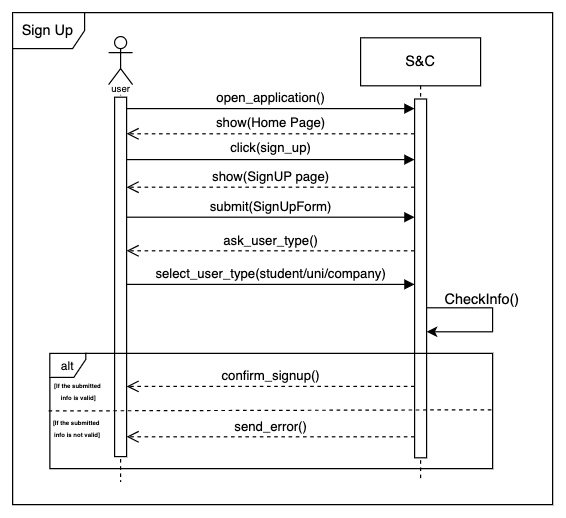
\includegraphics[width=0.7\textwidth]{Images/Sign_Up_Sequence_Diagram (5).png}
\caption{\label{fig:metamodel9}Sign Up Sequence Diagram.}
\end{figure}

\begin{figure}[H]
\centering
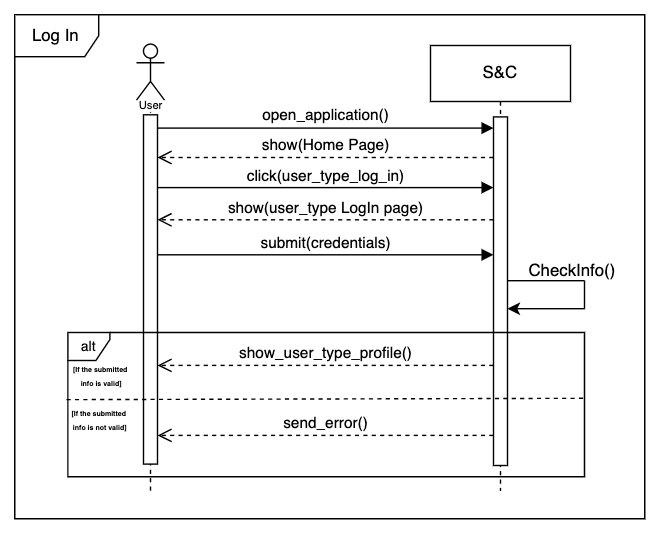
\includegraphics[width=0.7\textwidth]{Images/Log_In_Sequence_Diagram.png}
\caption{\label{fig:metamodel9}Log In Sequence Diagram.}
\end{figure}

\begin{figure}[H]
\centering
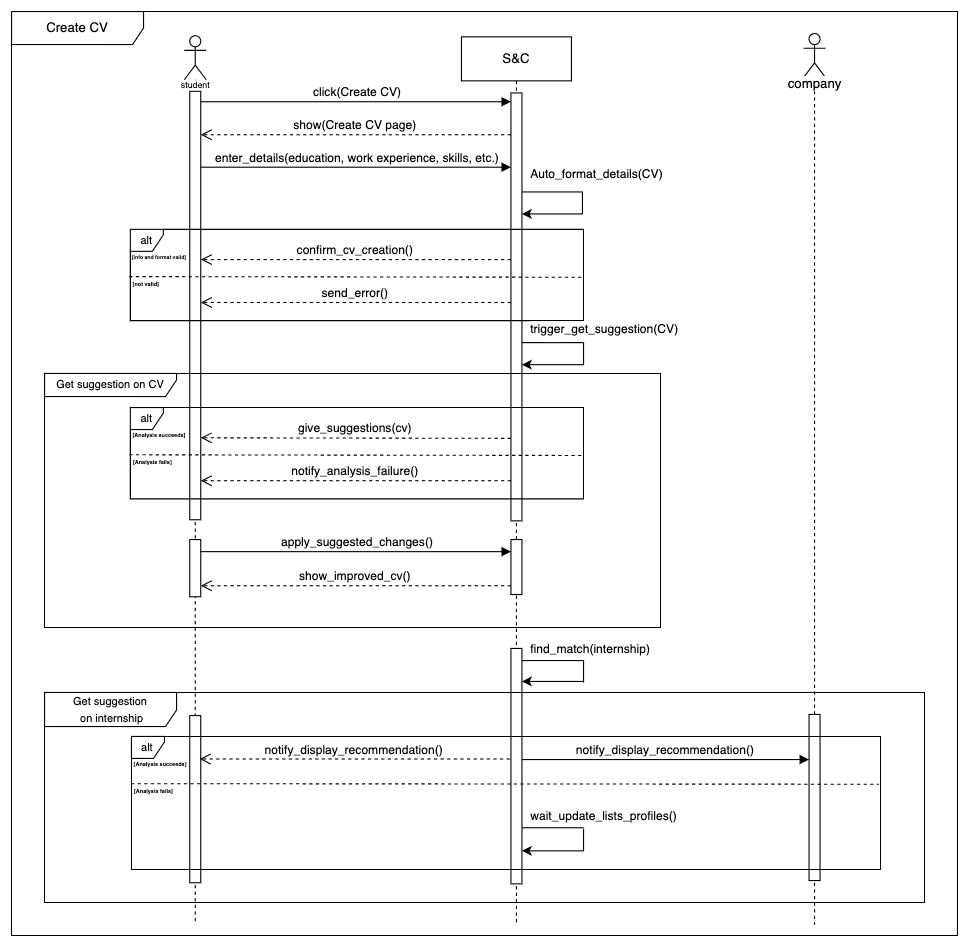
\includegraphics[width=0.8\textwidth]{Images/Create_CV_Sequence_Diagram (1).png}
\caption{\label{fig:metamodel9}Create CV Sequence Diagram.}
\end{figure}


\begin{figure}[H]
\centering
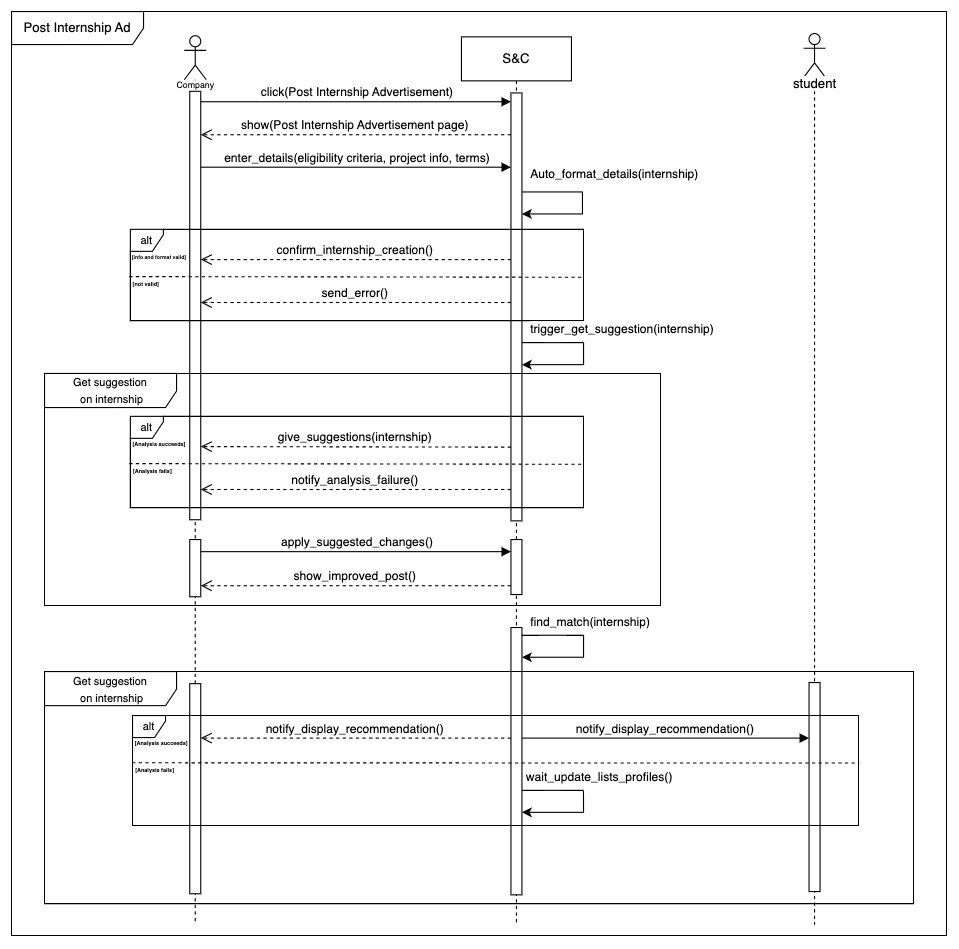
\includegraphics[width=0.8\textwidth]{Images/Post_Internship_Sequence_Diagram.png}
\caption{\label{fig:metamodel9}Post Internship Advertisement Sequence Diagram.}
\end{figure}


\begin{figure}[H]
\centering
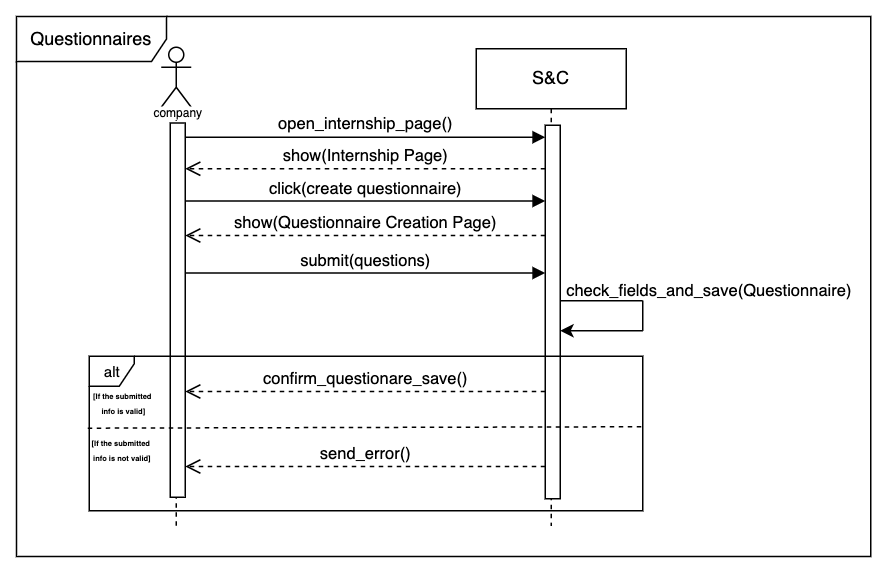
\includegraphics[width=0.8\textwidth]{Images/Questionnaire_Sequence_Diagram.png}
\caption{\label{fig:metamodel9}Questionnaire Creation Sequence Diagram.}
\end{figure}

\begin{figure}[H]
\centering
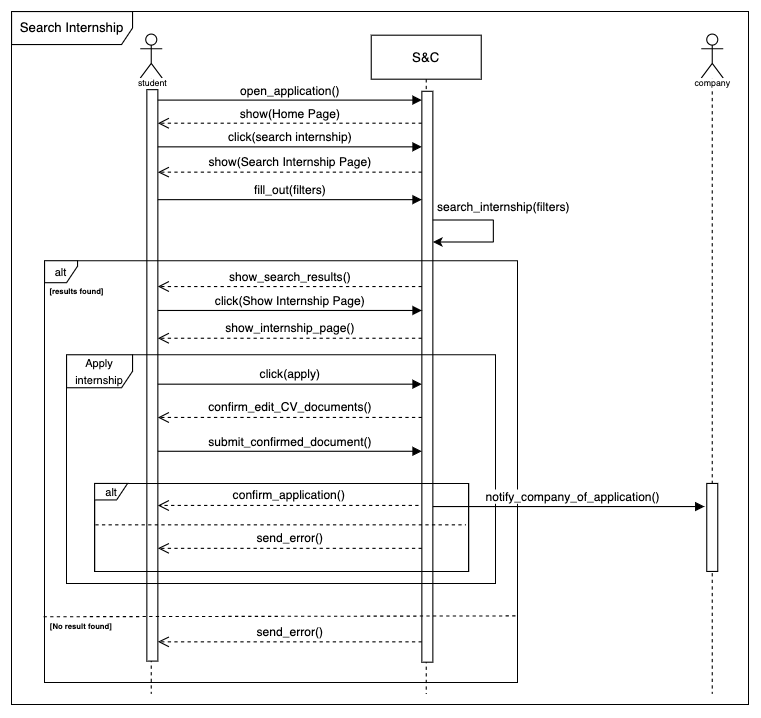
\includegraphics[width=0.8\textwidth]{Images/Internship_Search_Application_Sequence_Diagram.png}
\caption{\label{fig:metamodel9}Internship Search and Application Sequence Diagram.}
\end{figure}

\begin{figure}[H]
\centering
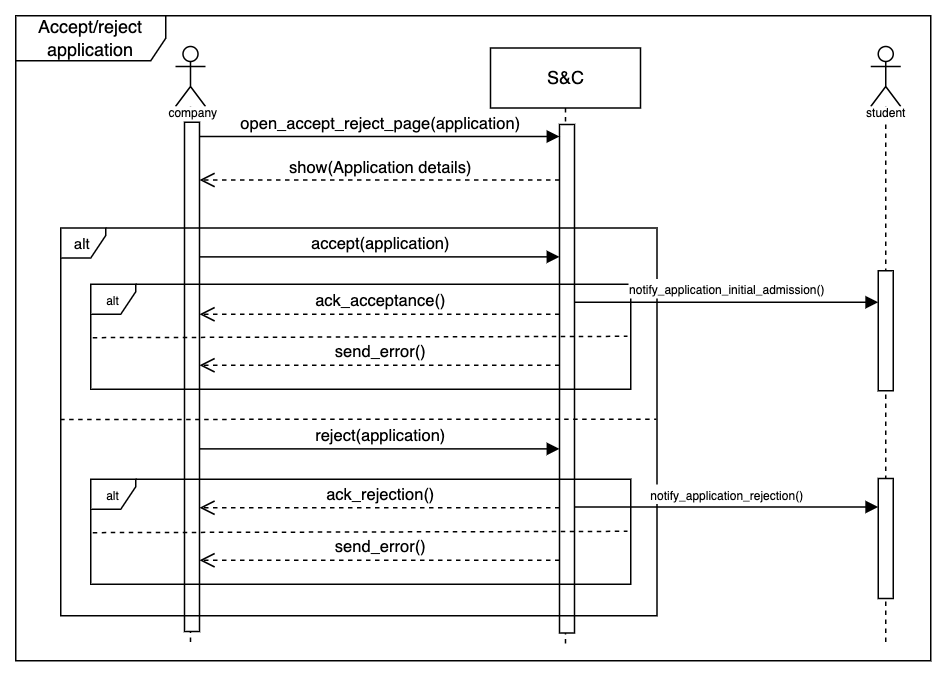
\includegraphics[width=0.8\textwidth]{Images/Accept_Reject_Application_Sequence_Diagram.png}
\caption{\label{fig:metamodel9}Accept or Reject Application Sequence Diagram.}
\end{figure}

\begin{figure}[H]
\centering
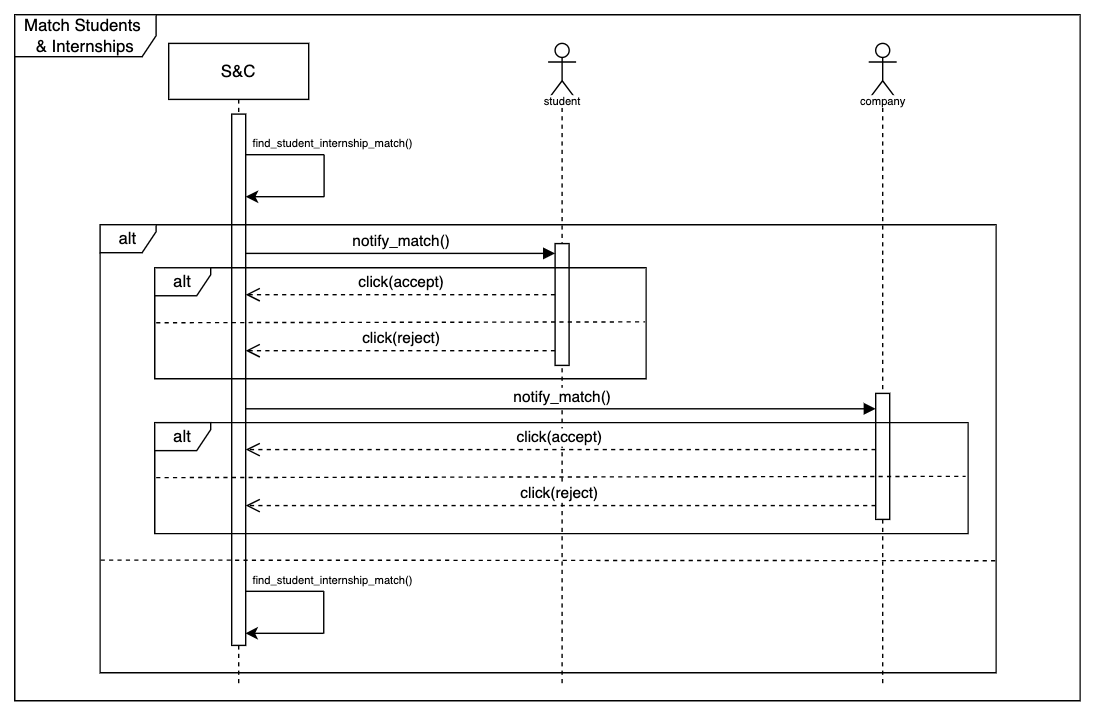
\includegraphics[width=0.8\textwidth]{Images/Match_Sequence_Diagram.png}
\caption{\label{fig:metamodel9}Match Student and Internship Sequence Diagram.}
\end{figure}

\begin{figure}[H]
\centering
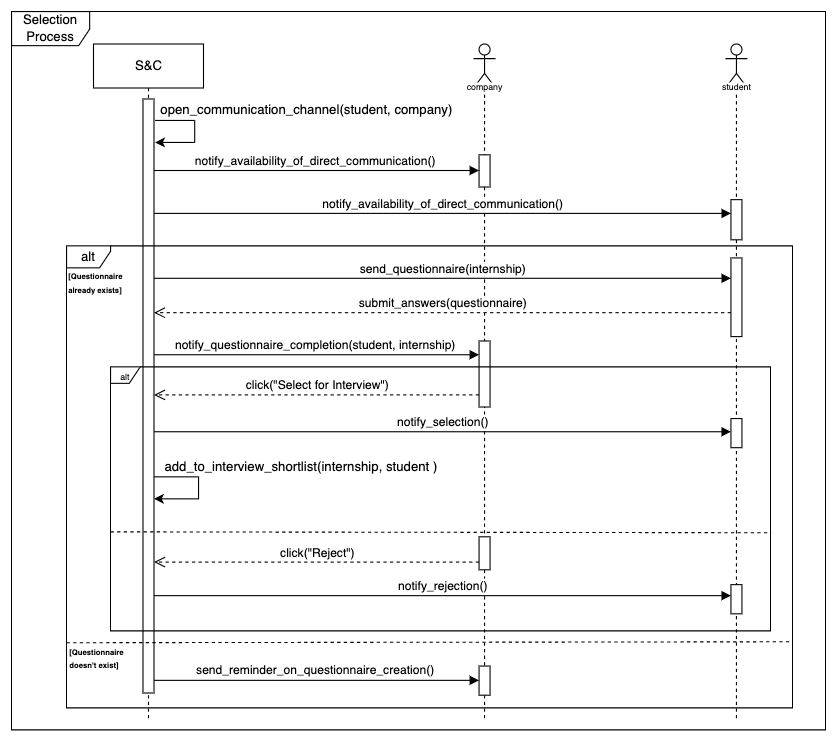
\includegraphics[width=0.8\textwidth]{Images/Selection_Process_Sequence_Diagram.png}
\caption{\label{fig:metamodel9}Selection Process Sequence Diagram.}
\end{figure}

\begin{figure}[H]
\centering
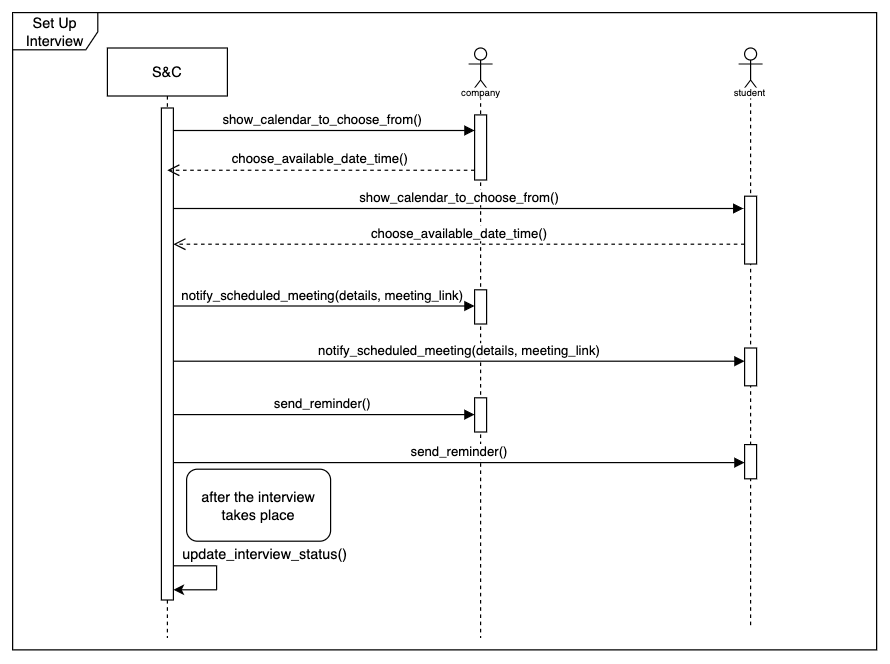
\includegraphics[width=0.8\textwidth]{Images/set_Up_Interview_Sequence_Diagram.png}
\caption{\label{fig:metamodel9}Set Up Interview Sequence Diagram.}
\end{figure}

\begin{figure}[H]
\centering
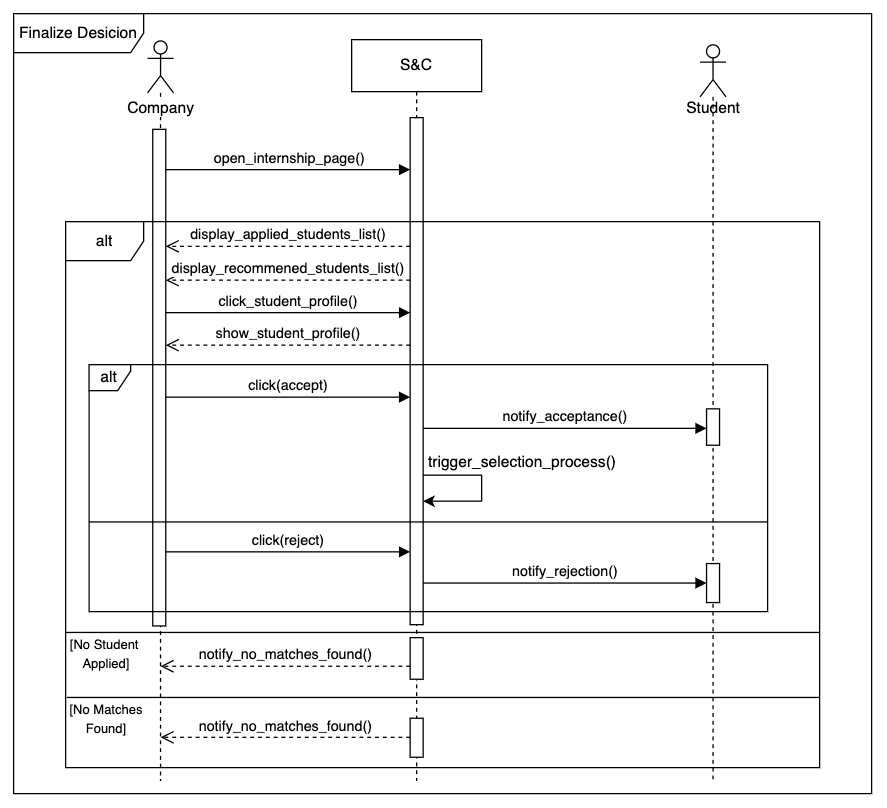
\includegraphics[width=0.8\textwidth]{Images/Finalize_Desicion_Sequence_Diagram.png}
\caption{\label{fig:metamodel9}Company Finalizing the decision on recruiting the student Sequence Diagram.}
\end{figure}

\begin{figure}[H]
\centering
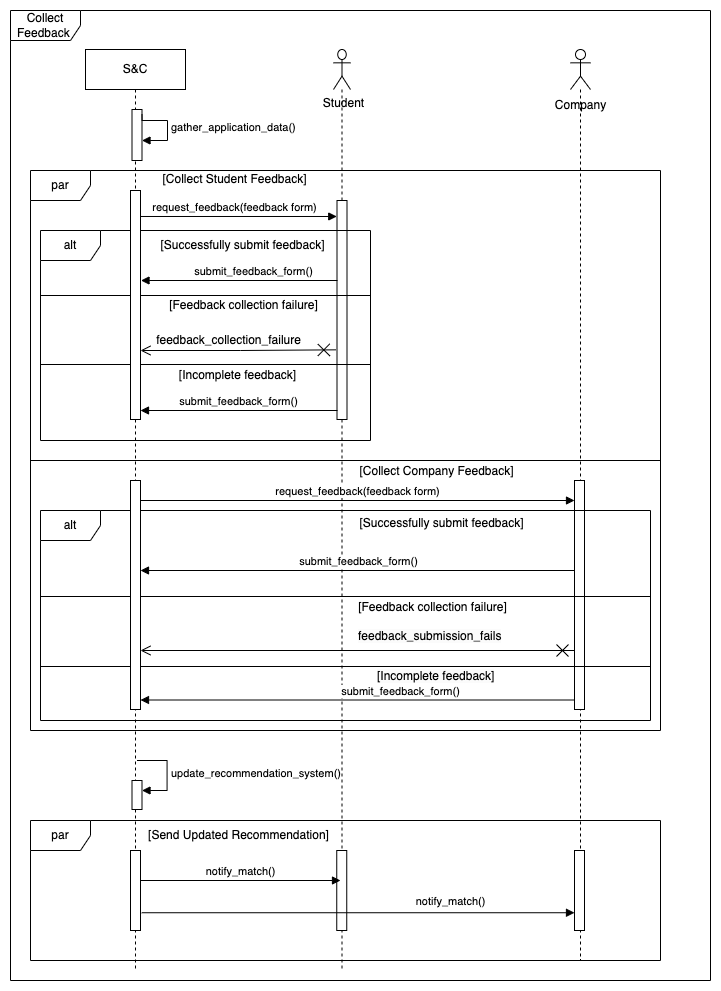
\includegraphics[width=0.8\textwidth]{Images/Collect_Feedback_Sequence_Diagram.png}
\caption{\label{fig:metamodel9}Collect Feedback Sequence Diagram}
\end{figure}

\begin{figure}[H]
\centering
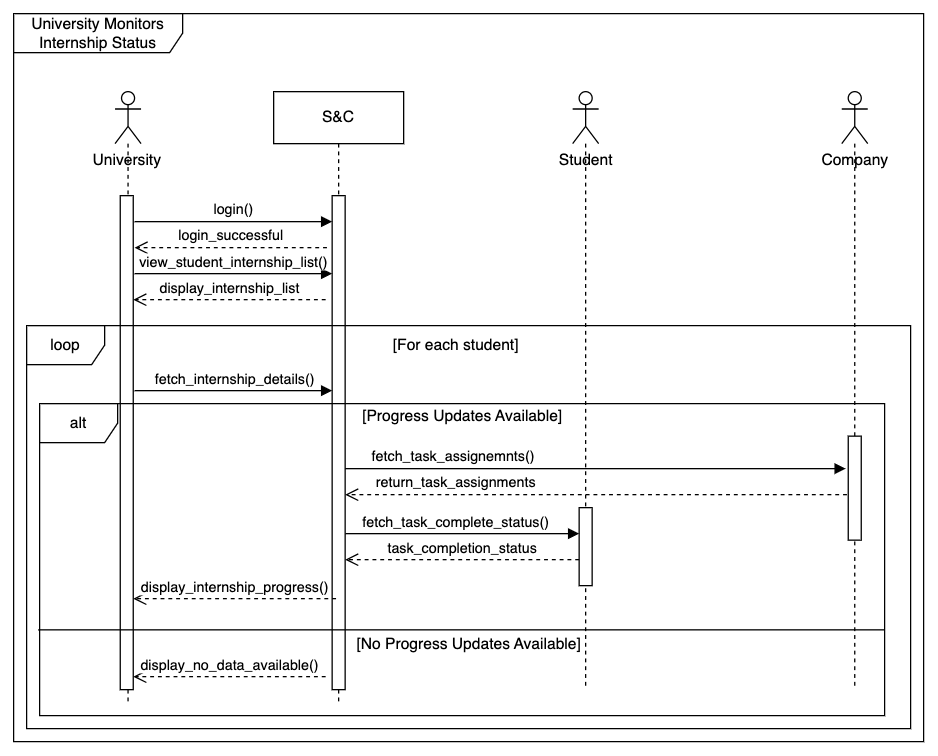
\includegraphics[width=0.8\textwidth]{Images/University_Monitor_Status_Sequence_Diagram.png}
\caption{\label{fig:metamodel9}University Monitors Internship Status Sequence Diagram}
\end{figure}

\begin{figure}[H]
\centering
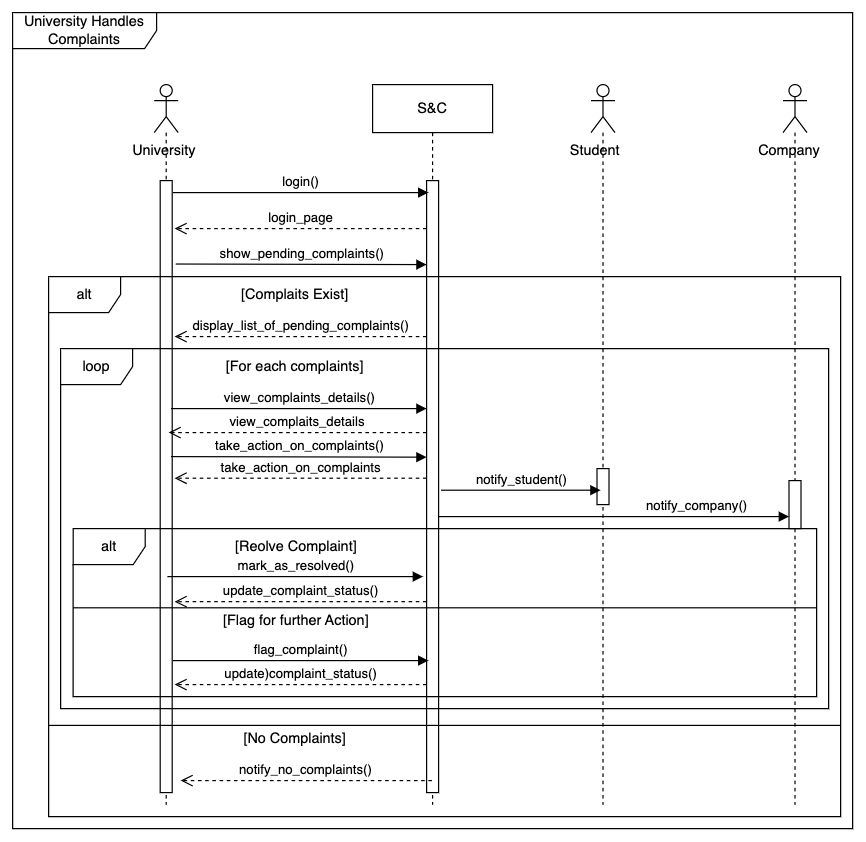
\includegraphics[width=0.8\textwidth]{Images/University_Handles_Complaints_Sequence_Diagram.png}
\caption{\label{fig:metamodel9}University Handles Complaints Sequence Diagram}
\end{figure}


\subsubsection{Requirement mapping}



\begin{xltabular}{\textwidth}{| l | X |}
\toprule
\multicolumn{2}{|c|}{G1}\\
\toprule
\textbf{G1} & \textbf{Allows registered students to create their profile and CV and search for internships and apply to them.}\\ [1ex]
\hline
D1 & The User must have a working Internet connection.\\ [1ex]
\hline
D2 & Student profiles are accurate and up-to-date. \\ [1ex]
\hline 
D3 & Internship availability is regularly updated. \\ [1ex]
\hline
D4 & Internship descriptions are clear and comprehensive. \\ [1ex]
\hline
D5 & Details provided by students and companies are true. \\ [1ex]
\hline
R1 & The S\&C system allows new users (students, universities and companies) to register by giving their credentials (e.g., name, email address, password). \\ [1ex]
\hline
R2 & The system allows users (students, universities and companies) to login. \\ [1ex]
\hline
R3 & The system allows students to create and update their profile (experience, skills, CV). \\ [1ex]
\hline
R6 & The system helps students in creating their CVs by giving intelligent suggestion for making a stronger CV and pointing out mistakes. \\ [1ex]
\hline
R7 & Students can search for internship opportunities clicking on "Search" button. \\ [1ex]
\hline
R8 & Students can apply to desired internship by clicking on "Apply" button for an internship post. \\ [1ex]
\hline
R9 & The system provides personalized recommendations to the students for internships based on students profiles and skills which matches with available internships. \\ [1ex]
\hline
R10 & Students can automatically apply to any recommended internship by clicking on "Accept" button. \\ [1ex]
\hline
\end{xltabular}

\begin{xltabular}{\textwidth}{| l | X |}
\toprule
\multicolumn{2}{|c|}{G2}\\
\toprule
\textbf{G2} & \textbf{Allows registered companies to create and post advertisement for available internship roles and select suitable candidate.}\\ [1ex]
\hline
D1 & The User must have a working Internet connection.\\ [1ex]
\hline
D2 & Student profiles are accurate and up-to-date. \\ [1ex]
\hline 
D3 & Internship availability is regularly updated. \\ [1ex]
\hline
D4 & Internship descriptions are clear and comprehensive. \\ [1ex]
\hline
D5 & Details provided by students and companies are true. \\ [1ex]
\hline
D6 & Student's eligibility for an internship is supervised by university. \\ [1ex]
\hline
R1 & The S\&C system allows new users (students, universities and companies) to register by giving their credentials (e.g., name, email address, password). \\ [1ex]
\hline
R2 & The system allows users (students, universities and companies) to login. \\ [1ex]
\hline
R4 & The system allows companies to create and update company's profile (about, field of work, achievements). \\ [1ex]
\hline
R11 & Companies can post internship opportunities and description which includes application domain, tasks to be performed, skills required. \\ [1ex]
\hline
R12 & The system can provide recommendations to improve the internship posts by companies. \\ [1ex]
\hline
R13 & The companies can prepare a questionnaire in the system to be forwarded to the students to get
additional information from them when the selection process starts. \\ [1ex]
\hline
R14 & The system can recommend companies about available students who match the job description and skills by applying statical analysis based on the characteristics of students and internships. \\ [1ex]
\hline
R15 & The system notifies students and companies once everyday to recommend new matches. \\ [1ex]
\hline
R16 & Companies can track applications and review candidate CVs. \\ [1ex]
\hline
R17 & Companies can accept or reject an application or a suggestion by the system by clicking on "Accept" or "Reject" buttons for each application. \\ [1ex]
\hline
R18 & A messaging channel is opened when a recommendation is accepted by both student and company or an application by student is accepted by company. \\ [1ex]
\hline
R19 & The prepared questionnaire is for forwarded to the student. \\ [1ex]
\hline
R20 & The system helps in management of the selection process by scheduling of interview. \\ [1ex]
\hline
R21& The system sends interview link or interview location to both student and company. \\ [1ex]
\hline
R22 & The system allows the company to update the interview results. \\ [1ex]
\hline
R23 & Interview results are updated in the platform and users are notified. \\ [1ex]
\hline
\end{xltabular}

\vspace{1.5em} % Optional space after the line

\begin{xltabular}{\textwidth}{| l | X |}
\toprule
\multicolumn{2}{|c|}{G3}\\
\toprule
\textbf{G3} & \textbf{Provide an efficient and intelligent matchmaking process between students and companies based on the students' skills and preferences, the companies' internship descriptions.}\\ [1ex]
\hline
D1 & The User must have a working Internet connection.\\ [1ex]
\hline
D2 & Student profiles are accurate and up-to-date. \\ [1ex]
\hline 
D3 & Internship availability is regularly updated. \\ [1ex]
\hline
D4 & Internship descriptions are clear and comprehensive. \\ [1ex]
\hline
D5 & Details provided by students and companies are true. \\ [1ex]
\hline
D6 & Student's eligibility for an internship is supervised by university. \\ [1ex]
\hline
D7 & Students and companies select their available times correctly during interview setup procedure. \\ [1ex]
\hline
R1 & The S\&C system allows new users (students, universities and companies) to register by giving their credentials (e.g., name, email address, password). \\ [1ex]
\hline
R2 & The system allows users (students, universities and companies) to login. \\ [1ex]
\hline
R3 & The system allows students to create and update their profile (experience, skills, CV). \\ [1ex]
\hline
R4 & The system allows companies to create and update company's profile (about, field of work, achievements). \\ [1ex]
\hline
R7 & Students can search for internship opportunities clicking on "Search" button. \\ [1ex]
\hline
R9 & The system provides personalized recommendations to the students for internships based on students profiles and skills which matches with available internships. \\ [1ex]
\hline
R10 & Students can automatically apply to any recommended internship by clicking on "Accept" button. \\ [1ex]
\hline
R11 & Companies can post internship opportunities and description which includes application domain, tasks to be performed, skills required. \\ [1ex]
\hline
R14 & The system can recommend companies about available students who match the job description and skills by applying statical analysis based on the characteristics of students and internships. \\ [1ex]
\hline
R15 & he system notifies students and companies once everyday to recommend new matches. \\ [1ex]
\hline
R17 & Companies can accept or reject an application or a suggestion by the system by clicking on "Accept" or "Reject" buttons for each application. \\ [1ex]
\hline
\end{xltabular}

\begin{xltabular}{\textwidth}{| l | X |}
\toprule
\multicolumn{2}{|c|}{G4}\\
\toprule
\textbf{G4} & \textbf{Support both students and companies during the selection process, including interview scheduling, questionnaire, feedback collection, and facilitating communication.}\\ [1ex]
\hline
D1 & The User must have a working Internet connection.\\ [1ex]
\hline
D2 & Student profiles are accurate and up-to-date. \\ [1ex]
\hline 
D3 & Internship availability is regularly updated. \\ [1ex]
\hline
D4 & Internship descriptions are clear and comprehensive. \\ [1ex]
\hline
D5 & Details provided by students and companies are true. \\ [1ex]
\hline
D6 & Student's eligibility for an internship is supervised by university. \\ [1ex]
\hline
D7 & Students and companies select their available times correctly during interview setup procedure. \\ [1ex]
R1 & The S\&C system allows new users (students, universities and companies) to register by giving their credentials (e.g., name, email address, password). \\ [1ex]
\hline
R2 & The system allows users (students, universities and companies) to login. \\ [1ex]
\hline
R13 & The companies can prepare a questionnaire in the system to be forwarded to the students to get
additional information from them when the selection process starts. \\ [1ex]
R18 & A messaging channel is opened when a recommendation is accepted by both student and company or an application by student is accepted by company. \\ [1ex]
\hline
R19 & he prepared questionnaire is for forwarded to the student.\\ [1ex]
\hline
R20 & The system helps in management of the selection process by scheduling of interview. \\ [1ex]
\hline
R21 & The system sends interview link or interview location to both student and company. \\ [1ex]
\hline
R22 & The system allows the company to update the interview results. \\ [1ex]
\hline
R23 & Interview results are updated in the platform and users are notified. \\ [1ex]
\hline
R24 & The system collects feedback from students and companies to then use the gathered data to better it's analysis and recommendation algorithm. \\ [1ex]
\hline
\end{xltabular}

\begin{xltabular}{\textwidth}{| l | X |}
\toprule
\multicolumn{2}{|c|}{G5}\\
\toprule
\textbf{G5} & \textbf{Allows registered universities to monitor the internship statuses of their students and take action on any issues or complaints.}\\ [1ex]
\hline
D1 & The User must have a working Internet connection.\\ [1ex]
\hline
D2 & Student profiles are accurate and up-to-date. \\ [1ex]
\hline 
D3 & Internship availability is regularly updated. \\ [1ex]
\hline
D4 & Internship descriptions are clear and comprehensive. \\ [1ex]
\hline
D5 & Details provided by students and companies are true. \\ [1ex]
\hline
D6 & Student's eligibility for an internship is supervised by university. \\ [1ex]
\hline
D7 & Students and companies select their available times correctly during interview setup procedure. \\ [1ex]
\hline
D8 & During complaint resolution process parties actually resolve the conflict. \\ [1ex]
\hline
R1 & The S\&C system allows new users (students, universities and companies) to register by giving their credentials (e.g., name, email address, password). \\ [1ex]
\hline
R2 & The system allows users (students, universities and companies) to login. \\ [1ex]
\hline
R3 & The system allows students to create and update their profile (experience, skills, CV). \\ [1ex]
\hline
R4 & The system allows companies to create and update company's profile (about, field of work, achievements). \\ [1ex]
\hline
R5 & The system allows universities to create and update their profile. \\ [1ex]
\hline
R25 & The system has a dedicated page to keep track and monitor all the ongoing search and selection processes for all three type of users (students, university, companies). \\ [1ex]
\hline
R26 & During the selection process and during interview the involved parties can raise concerns or complains which will be monitored by the university. \\ [1ex]
\hline
R27 & The system allows the university to decide on required actions to perform like warning to respective parties or interruption of internship and updates the same on the platform. \\ [1ex]
\hline
\end{xltabular}

\subsection{Performance Requirements}

The system shall ensure good performance in service of all kinds of users, including students, companies, and universities, efficiently. For usability, it shall meet the following minimum performance criteria:

The system should respond to user actions such as navigation or form submission in less than 1 second under normal conditions.
The system should support up to n users' concurrent access without significant degradation of performance, based on the number of students.

\subsection{Design Constraints}
\subsubsection{Standards compliance}
The Students\&Companies (S\&C) platform is conscious of and fully respects all data protection and security policies in light of the General Data Protection Regulation, otherwise known as the GDPR, along with assurances that guarantee data protection within the EU and EEA territories. It uses the modern international standard for date and time formatting.

\subsubsection{Hardware limitations}
The following hardware requirements are to be met by the user in order for the platform to work:

 - The devices should facilitate stable internet connectivity, ensuring at least one of the following standards: 3G, 4G, 5G, IEEE 802.11, or IEEE 802.3. The connections can be wired or wireless but reliable and maintain connectivity with the use of a modem, router, or any related device.
 - The hardware specifications of the devices need to be up-to-date, with a processor at least like Intel i5 or i7 and a display resolution not lower than Full HD. Besides, a minimum of 8 GB RAM is also essential for a smooth performance.
\subsubsection{Any other constraint}
The platform should be easy to handle by students and companies alike. The interface must support users at any level of technical skill so that searching for internships, submitting CVs, and tracking applications would be smooth and fast.


\subsection{Software System Attributes}

This section defines the non-functional requirements and software quality attributes that the Students\&Companies (S\&C) platform must meet to ensure reliability, security, and maintainability.

\subsubsection{Reliability}
 The system should support offline backups to recover from potential data loss and minimize disruption.
\subsubsection{Availability}
The system should be available to provide its functionalities with a minimum of 99.5\% uptime, meaning that the downtime is less than two days annually. Therefore, the platform should ensure redundancy for the critical components and perform scheduled maintenance during periods of low traffic.
\subsubsection{Security}
The platform should securely store user data, including the encryption of sensitive information like passwords and personal details. It shall use secure communication protocols, such as SSL/TLS, for securing data in transit from client to server. Then again, protection against internal and external threats should be good enough, with firewalls and intrusion detection systems amongst others. Besides, sensitive operations shall be restricted based on user role and permission.
\subsubsection{Maintainability}
The platform's codebase should be modular, well-documented, and easy to update. Clear comments and proper version control practices must be applied throughout the development lifecycle.
\subsubsection{Portability}
Being a web-based application, the platform should support the use of popular browsers like Google Chrome, Firefox, and Safari. It is also expected to be accessible via different devices: smartphones, tablets, and desktops.


